%%%%%%%%%%%%%%%%%%%%%%%%%%%%%%%%%%%%%%%%%%%%%%%%%%%
%% Author: Zbigniew Czarnecki 209909             %%
%% Latex scheme parent fork: tasklife-docs       %%
%% Latex scheme version: 0.2                     %%
%% + podzial na kolumny							 %%
%% + szablon wymagania funkcjonalne              %%
%% + szablon wymagania poza funkcjonalne         %%
%% + łamannie lini w tabular					 %%
%% + ryyko										 %%
%%%%%%%%%%%%%%%%%%%%%%%%%%%%%%%%%%%%%%%%%%%%%%%%%%%

\documentclass[a4paper, 11pt]{article}
\usepackage[margin=2.5cm]{geometry}

\usepackage[T1]{fontenc}
\usepackage[utf8]{inputenc}
\usepackage[english, polish]{babel}

%wciecie pierwszego wiersza
\usepackage{indentfirst}
\setlength{\parindent}{1cm}

%ładne linki (nie rzuca się o podkreślenia i procenty)
\usepackage{hyperref}

%manipulacje kolumną w tabeli (pogrubienie tekstu w całej kolumnie)
\usepackage{array}

%tabele na do maksymalnej szerokosci strony
\usepackage{tabularx}

%dodawanie plików graficznych
\usepackage{graphicx}

%lepsza czcionka do latexa
\usepackage{times}

%podział na kolumny
\usepackage{multicol}

%w tej komurce można łamać linie "\\"
\usepackage{makecell}

%%% Schematy

%tłusty tekst, do lewej
\newcolumntype{R}[1]{>{\raggedright\bfseries}p{#1}}
%do lewej
\newcolumntype{L}[1]{>{\raggedright}p{#1}}

%% Wymagania funckjonalne

% 
\def\funcreq#1#2#3#4#5#6#7#8#9{%
	\def\funcreqcontinued##1{%
		\vspace{0.2cm}
		\begin{tabularx}{\textwidth}{|R{4cm}|L{11.1cm}|}
			\hline
			Nr wymagania & #1 \tabularnewline \hline
			Nazwa & #2 \tabularnewline \hline
			Opis & #3 \tabularnewline \hline
			Przesłanka & #4 \tabularnewline \hline
			Ograniczenia i warunki & #5 \tabularnewline \hline
			Dane wejściowe & #6 \tabularnewline \hline
			Źródło danych & #7 \tabularnewline \hline
			Wynik & #8 \tabularnewline \hline
			Priorytet & #9 \tabularnewline \hline
			Kryterium do spełnienia & ##1 \tabularnewline \hline
		\end{tabularx}
		\vspace{0.2cm}
	}%
	\funcreqcontinued%
}

%Przyklad: \funcreq{Nr wymagania}{Nazwa}{Opis}{Przesłanka}{Ograniczenia i warunki}{Dane wejściowe}{Źródło danych}{Wynik}{Priorytet}{Kryterium do spełnienia}

%\funcreq{
%		1
%	}{
%		Nazwa
%	}{
%		Opis
%	}{
%		Przesłanka
%	}{
%		Ograniczenia i warunki
%	}{
%		Dane wejściowe
%	}{
%		Źródło danych
%	}{
%		Wynik
%	}{
%		Priorytet
%	}{
%		Kryterium do spełnienia
%}

%% Wymagania poza funkcjonalne

\newcommand{\nonefuncreq}[5]{
	\vspace{0.2cm}
	\begin{tabularx}{\textwidth}{|R{4cm}|L{11.1cm}|}
		\hline
		Nr wymagania & #1 \tabularnewline \hline
		Nazwa & #2 \tabularnewline \hline
		Opis & #3 \tabularnewline \hline
		Przesłanka & #4 \tabularnewline \hline
		Kryterium do spełnienia & #5 \tabularnewline \hline
	\end{tabularx}
	\vspace{0.2cm}
}

%Przyklad: \nonefuncreq{Nr wymagania}{Nazwa}{Opis}{Przesłanka}{Kryterium do spełnienia}

%\nonefuncreq{
%		1
%	}{
%		Nazwa
%	}{
%		Opis
%	}{
%		Przesłanka
%	}{
%		Kryterium do spełnienia
%}

%% Ryzyka

\newcommand{\risk}[5]{
	\vspace{0.2cm}
	\begin{tabularx}{\textwidth}{|R{4cm}|L{11.1cm}|}
		\hline
		Zagrożenie & #1 \tabularnewline \hline
		Skutek & #2 \tabularnewline \hline
		Prawdopodobieństwo wystąpienia & #3 \tabularnewline \hline
		Ryzyko & #4 \tabularnewline \hline
		Profilaktyka & #5 \tabularnewline \hline
	\end{tabularx}
	\vspace{0.2cm}
}

%\risk{
%	Zagrożenie
%}{
%	Skutek
%}{
%	Prawdopodobieństwo wystąpienia
%}{
%	Ryzyko
%}{
%	Profilaktyka
%}

%Przyklad: \risk{Zagrożenie}{Skutek}{Prawdopodobieństwo wystąpienia}{Ryzyko}{Profilaktyka}

\begin{document}

\begin{titlepage}
	
	\begin{center}
		\huge{\uppercase{\textbf{Politechnika Wrocławska}}}
	\end{center}

	\begin{flushright}
		Wrocław, 30 październik 2017
	\end{flushright}

	\vspace{2cm}
	\begin{flushleft}
		\textbf{\\
			Wydział Elektroniki\\
			Kierunek: Informatyka\\
			Semestr: 2017/18 ZIMA\\
			Prowadzący: dr inż. Konrad Jackowski \\
		}
	\end{flushleft}
	
	\vspace{3cm}
	\begin{center}
		\textbf{
			\huge{\uppercase{Projektowanie telemedycznych systemów internetowych i~mobilnych}}\\
			\LARGE{projekt}
		}\\
		\huge{Temat: Aplikacja do zarządzania dniem pracy specjalistów oraz rejestracji pacjentów w~zakładzie rehabilitacji}
	\end{center}
	
	\vspace{5cm}
	\begin{multicols}{2}
		\begin{tabularx}{\textwidth}{ll}
			Zbigniew Czarnecki & 209909 \\
			Maksymilian Iwanow & 209946 \\
			Mateusz Ligus & 209939 \\
		\end{tabularx}
		\columnbreak
		\begin{tabularx}{\textwidth}{ll}
			Marcin Pawłowski & 218441 \\
			Jakub Sanecki & 210016 \\		
			Piotr Wolf & 210036 \\
		\end{tabularx}
	\end{multicols}

\end{titlepage}

\tableofcontents
\section{Specyfikacja wymagań}

\subsection{Czynniki sterujące projektem}

\subsubsection{Cele projektu}

\begin{itemize}
	\item Wdrożenie aplikacji do zarządzania dniem pracy specjalistów
	i~przypisywania im sprzętu rehabilitacyjnego na określoną porę,
	\begin{itemize}
		\item 30\% zwiększenie efektywności pracy poprzez usprawnienie systemu przypisywania specjalistom dostępu do sprzętu rehabilitacyjnego, maksymalnie pokrywając ich czas pracy zajęciami,
	\end{itemize}
	\item Wdrożenie systemu do rejestracji pacjentów,
	\begin{itemize}
		\item 50\% zmniejszenie kosztów obsługi rejestracji pacjentów, poprzez automatyzację tej procedury, co umożliwi redukcję etatów pracowników recepcji.
	\end{itemize}
\end{itemize}

\subsubsection{Użytkownicy produktu}

\begin{itemize}
	\item Klient
	\begin{itemize}
		\item Obsługa zakładu rehabilitacyjnego, administrująca czasem pracy specjalistów jak i~dostępem do sal.
	\end{itemize}
	\item Użytkownicy
	\begin{itemize}
			\item Wszyscy potencjalni klienci rejestrujący się na zajęcia rehabilitacyjne.
	\end{itemize}
\end{itemize}


\subsection{Czynniki sterujące projektem}

\subsubsection{Cele projektu}

\begin{itemize}
	\item Wdrożenie aplikacji do zarządzania dniem pracy specjalistów
	i~przypisywania im sprzętu rehabilitacyjnego na określoną porę,
	\begin{itemize}
		\item 30\% zwiększenie efektywności pracy poprzez usprawnienie systemu przypisywania specjalistom dostępu do sprzętu rehabilitacyjnego, maksymalnie pokrywając ich czas pracy zajęciami,
	\end{itemize}
	\item Wdrożenie systemu do rejestracji pacjentów,
	\begin{itemize}
		\item 50\% zmniejszenie kosztów obsługi rejestracji pacjentów, poprzez automatyzację tej procedury, co umożliwi redukcję etatów pracowników recepcji.
	\end{itemize}
\end{itemize}

\subsubsection{Użytkownicy produktu}

\begin{itemize}
	\item Klient
	\begin{itemize}
		\item Obsługa zakładu rehabilitacyjnego, administrująca czasem pracy specjalistów jak i~dostępem do sal.
	\end{itemize}
	\item Użytkownicy
	\begin{itemize}
			\item Wszyscy potencjalni klienci rejestrujący się na zajęcia rehabilitacyjne.
	\end{itemize}
\end{itemize}

\subsection{Ograniczenia projektu}

\subsubsection{Ograniczenia wynikające z natury i~okoliczności projektu}

\begin{itemize}
	\item Wszystkie dane klientów muszą podlegać ochronie zgodnie z ustawą o~ochronie danych osobowych (Dz.U. 1997 Nr 133 poz. 883),
	\item Aplikacja ma zostać wykonana w formie aplikacji webowej,
	\item Do działania aplikacji konieczne jest połączenie z internetem,
	\item Wszystkie prace projektowe powinny zostać zaplanowane tak, aby umożliwić uruchomienie i~pełne funkcjonowanie systemu do 1~grudnia~2017~roku,
Brak funduszy, ponieważ jest to projekt studencki.
	%TODO
	\item Dodałbym jeszcze ograniczenie związane z technologią czyli Yii2 jak mniemam. Zbychu bardziej sie znasz to możesz ładnie sformułować.
\end{itemize}

\subsubsection{Konwencje nazewnicze i~definicje}
%TODO !!!!! Tutaj trzeba wstawić wszystkie akronimy i skróty myślowe które popełnimy w tym dokumencie !!!
\begin{itemiz}
	\item \textit{Aplikacja webowa} - program znajdujący się na serwerze komunikujący się z użytkownikiem za pomocą przeglądarki internetowej,
	\item \textit{Przeglądarka internetowa} - program służący do wyświetlania aplikacji webowych,
	\item \textit{Logowanie} - proces autoryzacji użytkownika polegający podaniu identyfikatora i~hasła,
\end{itemize}

\subsubsection{Fakty i~założenia powiązane z~projektem}
\begin{itemize}
	\item Witryna ma być zaprojektowana w taki sposób, aby nie sprawiać trudności podczas rejestracji pacjentów.
	\item Należy założyć, że z~witryny mogą korzystać zarówno osoby starsze jak i~młodsze, interfejs powinien być intuicyjny aby obsłużyć go mogły osoby niedoświadczone jak i~aby osoby obyte z~tego typu narzędziami mogły szybko wykonać chciane operacje. %TODO paskudny język
\end{itemize}

\section{Elementy zarządzania projektem}

\subsection{Harmonogram projektu}

Prace projektowe zostały podzielone na 3 etapy:
\begin{itemize}
	\item Burza mózgów, tworzenie wymagań, wybór technologii, specyfikacja architektury. 
	\item Podział modułowy, implementacja rozwiązań.
	\item Poprawki, testy, tworzenie podsumowania.
\end{itemize}

\begin{tabularx}{\textwidth}{|p{1cm}|p{4cm}|p{9.68cm}|}
	\hline
	Etap & Termin & Podetapy \tabularnewline \hline
	I & 4.10.2017 - 30.10.2017 &
		\begin{enumerate}
			\item Wybór tematu.
			\item Burza mózgów – ustalanie wykorzystywanej technologii, podstawowych funkcjonalności. 
		\end{enumerate}
		\tabularnewline \hline
	II & 30.10.2017 - 12.11.2017 &
		\begin{enumerate}
			\item Instalacja środowisk na stacjach roboczych członków grupy.
			\item Konfiguracje środowisk.
			\item Szkolenie zespołu pod katem wykorzystanych technologi.
			\item Zapoznanie się ze zrozumieniem członków zespołu z dokumentacją projektu.
			\item Rozpoczęcie pracy nad implementacją projektu.
		\end{enumerate}
	\tabularnewline \hline
	III & 12.10.2017 - 19.11.2017 &
	\begin{enumerate}
		\item Implementacja bazy danych.
		\item Systemy autoryzacji modułów administratora, klienta i~lekarza.
		\item Modelowanie bazy danych i~połączenie jej systemem ORM.
		\item Implementacja CRUD'ÓW Sprzętu, Zabiegów i Lekarzy.
		\item Rozpoczęcie pracy nad aplikacją mobilną.
		\item Rozpoczęcie pracy nad implementacją modułu dla pacjenta.
	\end{enumerate}
	\tabularnewline \hline
	IV & 20.11.2017 - 26.12.2017 &
		\begin{enumerate}
			\item Implementacja kalendarza terminów.
			\item Implementacja API wykorzystywanego przez aplikację mobilną.
			\item Implementacja użycia API w aplikacji mobilnej.
			\item Ukończenie modułu dla pacjenta.
		\end{enumerate}
	\tabularnewline \hline
\end{tabularx}
\begin{tabularx}{\textwidth}{|p{1cm}|p{4cm}|p{9.68cm}|}
	\hline
	V & 27.11.2017 - 03.12.2017 &
	\begin{enumerate}
		\item Ukończenie aplikacji mobilnej.
		\item Ukończenie modułu administracyjnego.
		\item Implementacja użycia API w aplikacji mobilnej.
		\item Testowanie.
		\item Wzbogacenie dokumentacji projektowej o~wnioski i~przemyślenia.
		\item Oddanie projektu.
	\end{enumerate}
	\tabularnewline \hline
\end{tabularx}

\subsection{Podział zasobów}

W celu właściwego przygotowania i~wdrożenia projektu został opracowany odpowiedni podział zasobów ludzkich oraz czasowych. Umożliwi on sprawne zarządzanie przedsięwzięciem, kontrolę zgodności rozwiązań oraz nadzór lidera projektu nad terminowością realizowanych zadań. Ze względu na krótki okres trwania projektu, niezbędne było wprowadzenie rygoru pracy, ściśle związanego z wyznaczonym harmonogramem.Podział zasobów

\begin{itemize}
	\item Odgórny nadzór nad projektem sprawowany jest przez dr inż. Konrada Jackowskiego - prowadzącego projekt,
	\item Operacyjne zarządzanie przedsięwzięciem sprawowane jest przez lidera grupy - Zbigniewa Czarneckiego. Do jego obowiązków należy informowanie opiekuna projektu o postępie prac, przeprowadzanych modyfikacjach, napotkanych problemach oraz rozdzielanie zadań w obrębie grupy,
	\item Poszczególne moduły projektowe realizowane są przez wszystkich członków zespołu, podzielonych na dwuosobowe podgrupy:
	\begin{itemize}
		\item 
	\end{itemize}
\end{itemize}



\begin{tabular}{|p{7.7cm}|l|l|}
	\hline
	Moduł & Podgrupa & Termin wykonania \tabularnewline \hline
	Moduł zarządzania lekarzami i~zasobami placówki & \makecell[l]{Maksymilian Iwanow \\ Piotr Wolf} & 17.11.2017 \tabularnewline \hline
	Moduł wyszukiwania lekarzy oraz zabiegów w~zakładzie rehabilitacji & \makecell[l]{Mateusz Ligus \\ Marcin Pawłowski} & 16.11.2017 \tabularnewline \hline
	Moduł rejestracji pacjentów na zabiegi & \makecell[l]{Zbigniew Czarnecki (lider) \\ Jakub Sanecki} & 18.11.2017 \tabularnewline \hline
\end{tabular}

\subsection{Analiza ryzyka}

\risk{
	Przekroczenie planowanego terminu oddania projektu.
}{
	Obniżona ocena bądź brak zaliczenia z przedmiotu PTSIM.
}{
	Duże.
}{
	Wysokie.
}{
	Cykliczne spotkania zespołu projektowego, omawianie postępów i problemów, określenie ram czasowych na wykonanie poszczególnych zadań projektowych.
}

\risk{
	Awarie techniczne sprzętu.
}{
	Brak możliwości tworzenia/rozwijania oprogramowania/utrata danych.
}{
	Średnie.
}{
	Średnie.
}{
	Konserwacja i odpowiednie zabezpieczanie sprzętu.
}

\risk{
	Problemy z komunikacją w zespole.
}{
	Członkowie grupy nie wiedzą, czym powinni się zająć.
}{
	Małe.
}{
	Średnie.
}{
	Stworzenie wielu kanałów komunikacji (internet, telefon, spotkania), kontrola każdego członka zespołu przez lidera.
}

\risk{
	Brak umiejętności pracy w grupie przez członków zespołu. Brak doświadczenia w pracy grupowej u członków zespołu
}{
	Opóźnienia w tworzeniu modułów, tworzenie się podgrup wśród członków zespołu.
	Opóźnienia w tworzeniu modułów, tworzenie się podgrup wśród członków zespołu mających inny pomysł wykonania projektu czego wynikiem może być rozłam grupy
	
}{
	Małe.
}{
	Małe.
}{
	Tworzenie przyjaznej atmosfery, organizowanie wyjść integracyjnych.
}

\risk{
	Niedoświadczony zespół projektowy. 
}{
	Opóźnienia, słaba jakość kodu, produkt nie spełnia założonych wymogów.
}{
	Duże.
}{
	Wysokie.
}{
	Doszkalanie grupy z nieznanych im technologii.
}

\risk{
	Niedyspozycyjność członka grupy projektowej.
}{
	Trudność w podziale zadań.
}{
	Duże.
}{
	Średnie.
}{
	Niedyspozycyjnosć jest najczęściej spowodowana zdarzeniem czysto losowym - ciężko ją przewidzieć jak i jej przeciwdziałać.
}

\risk{
	Utrata fragmentów kodu.
}{
	Konieczność tworzenia rozwiązań od nowa.
}{
	Małe.
}{
	Średnie.
}{
	Kod przechowywany w wielu miejscach, wykorzystanie repozytorium.
}

\risk{
	Zdefiniowanie niepotrzebnych wymagań.
}{
	Podrzędne cele zabierają za dużo czasu, którego może zabraknąć do osiągnięcia sukcesu.
}{
	Średnie.
}{
	Małe.
}{
	Jasno określony czas pracy nad konkretnymi modułami.
}

\risk{
	Zmiana wymagań klienta w trakcie tworzenia oprogramowania.
}{
	Redefinicja projektu, możliwość jego upadku.
}{
}{
	Wysokie.
}{
	Wyznaczenie stałych terminów na wprowadzanie ewentualnych poprawek bądź nowych funkcjonalności.
}

\risk{
	Wycofanie się klienta z projektu.
}{
	Upadek projektu.
}{
	Małe.
}{
	Wysokie.
}{
	Stały kontakt z klientem, umowa nakładająca karę na klienta w wypadku wycofania się z projektu w celu zapewnienia funduszy zapobiegających upadkowi firmy.
}


\section{Opis realizowanej aplikacji}

\subsection{Moduł aministracyjny}

\begin{itemize}
	\item Wymagania funkcjonalne dotyczące modułu administracyjnego zostały opisane w sekcji 1.3.1. Pierwsze pięć z nich dotyczą czynności związanych z autoryzacją administratora. Użytkownikowi posiadającemu status administratora, aplikacja umożliwia logowanie, resetowanie hasła w przypadku jego utraty, zmianę hasła i adresu email, gdy administrator jest już zalogowany, oraz wylogowanie. Widoki umożliwiające dokonanie ww. działań zostały przedstawione poniżej. 

\vspace{0,5cm}
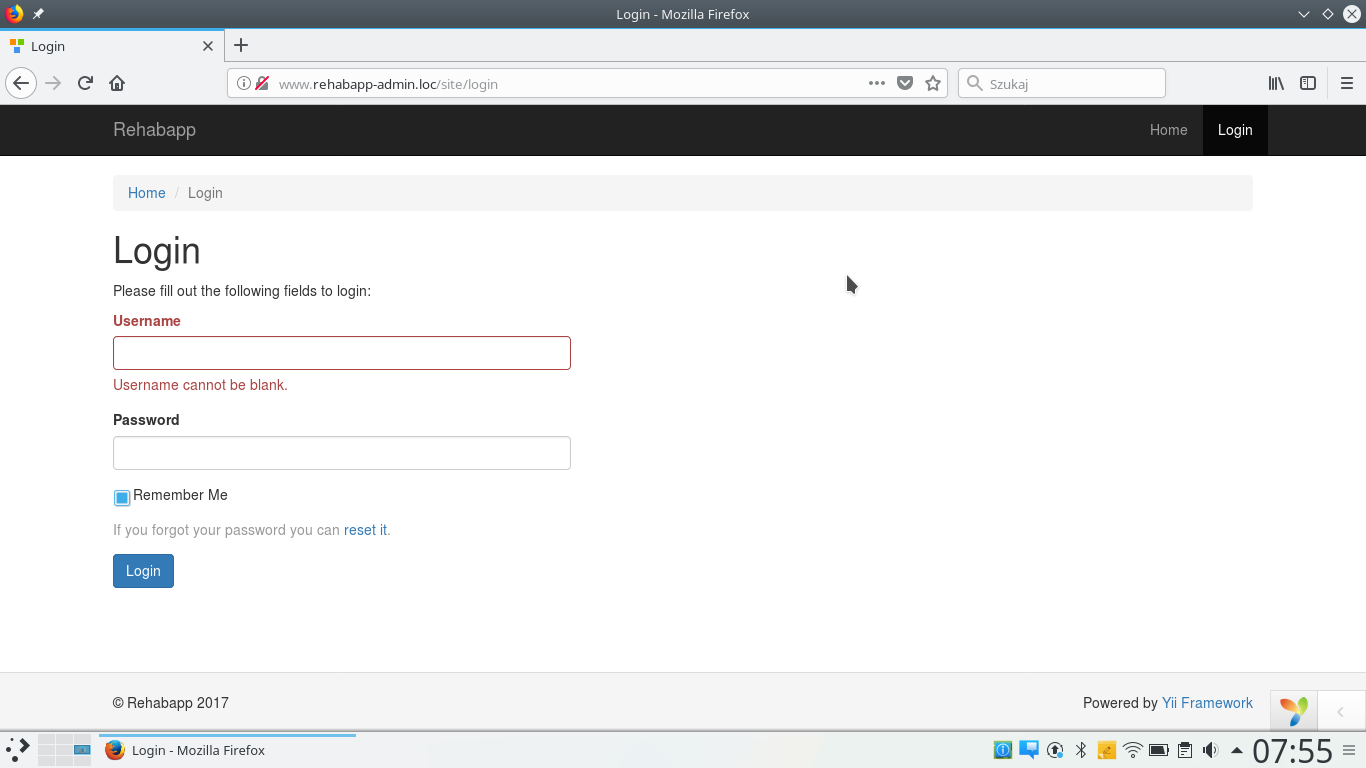
\includegraphics[scale=0.4]{obraz/1.png}
%\begin{center}{\scriptsize Rysunek 1: Diagram przypadków użycia.}\end{center}
\vspace{0,5cm}

\vspace{0,5cm}
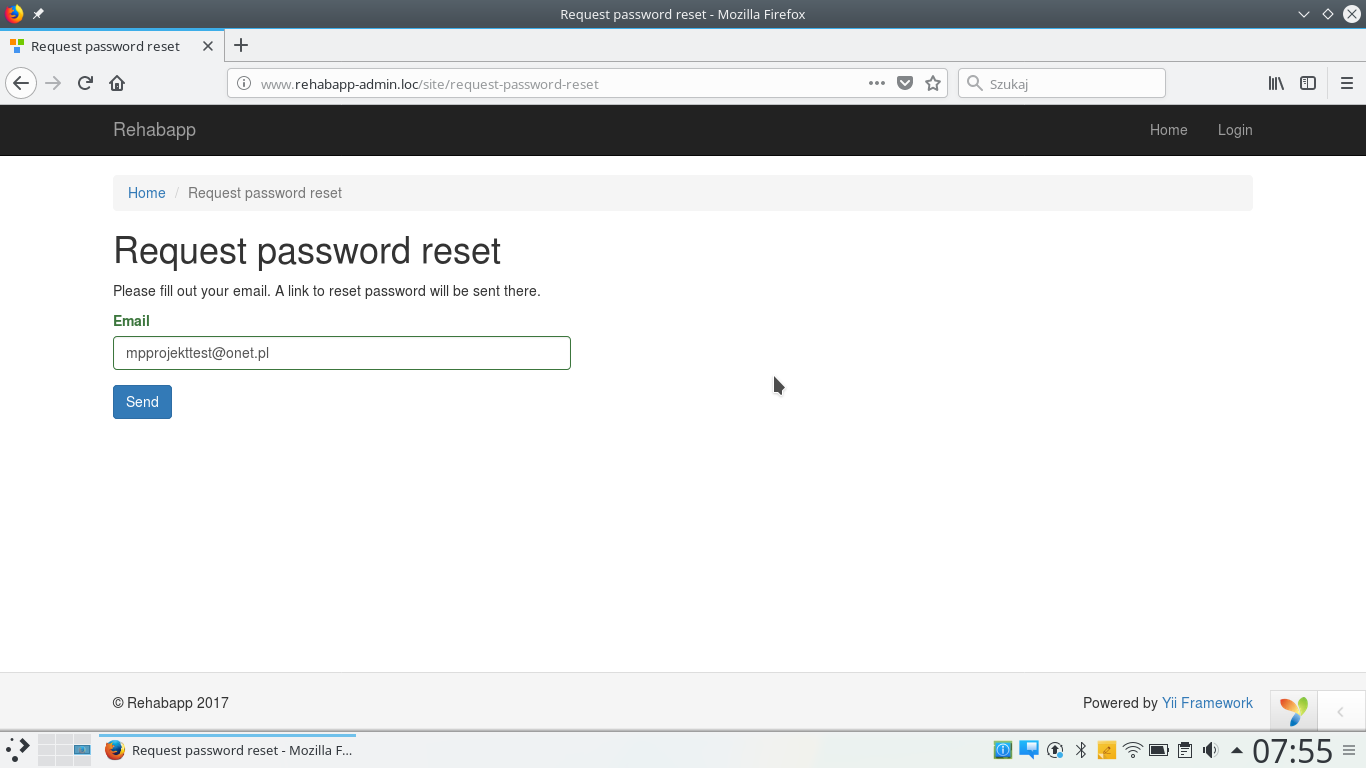
\includegraphics[scale=0.4]{obraz/2.png}
%\begin{center}{\scriptsize Rysunek 1: Diagram przypadków użycia.}\end{center}
\vspace{0,5cm}

\vspace{0,5cm}
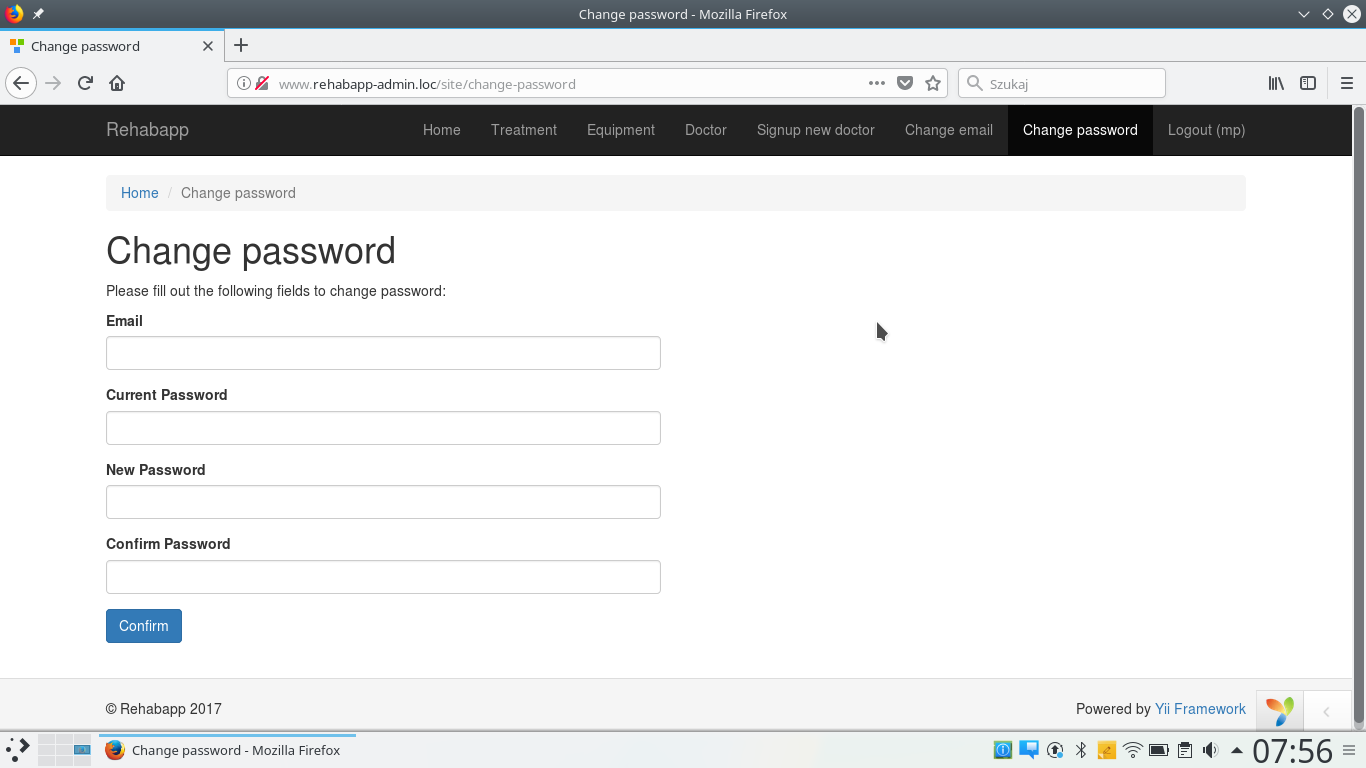
\includegraphics[scale=0.4]{obraz/3.png}
%\begin{center}{\scriptsize Rysunek 1: Diagram przypadków użycia.}\end{center}
\vspace{0,5cm}

\vspace{0,5cm}
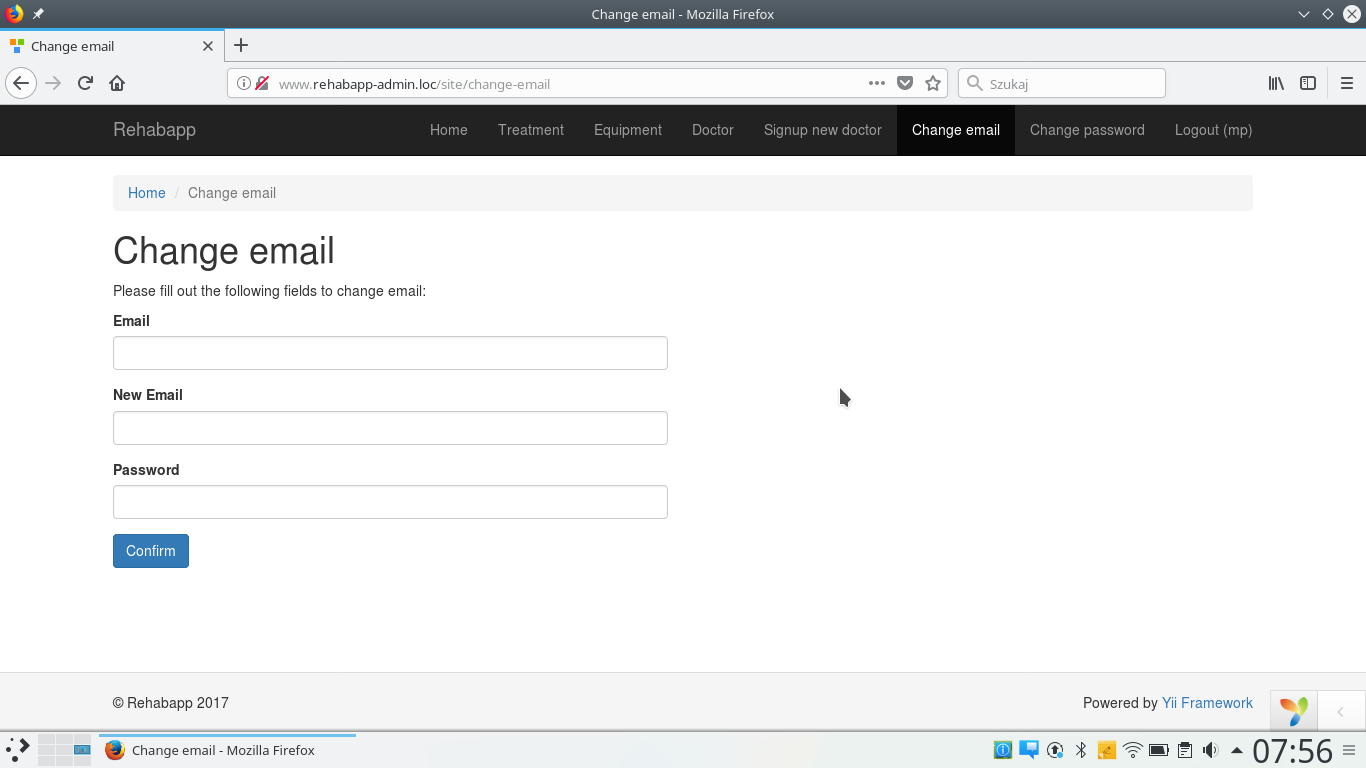
\includegraphics[scale=0.4]{obraz/4.png}
%\begin{center}{\scriptsize Rysunek 1: Diagram przypadków użycia.}\end{center}
\vspace{0,5cm}
\newpage
	\item Kolejne 5 wymagań dotyczyło zarządzania zasobami placówki. System umożliwia dodawanie, edycję, usuwanie, wyświetlanie szczegółów dotyczących sprzętu oraz listę wszystkich zapisanych w bazie zasobów.
	
\vspace{0,5cm}
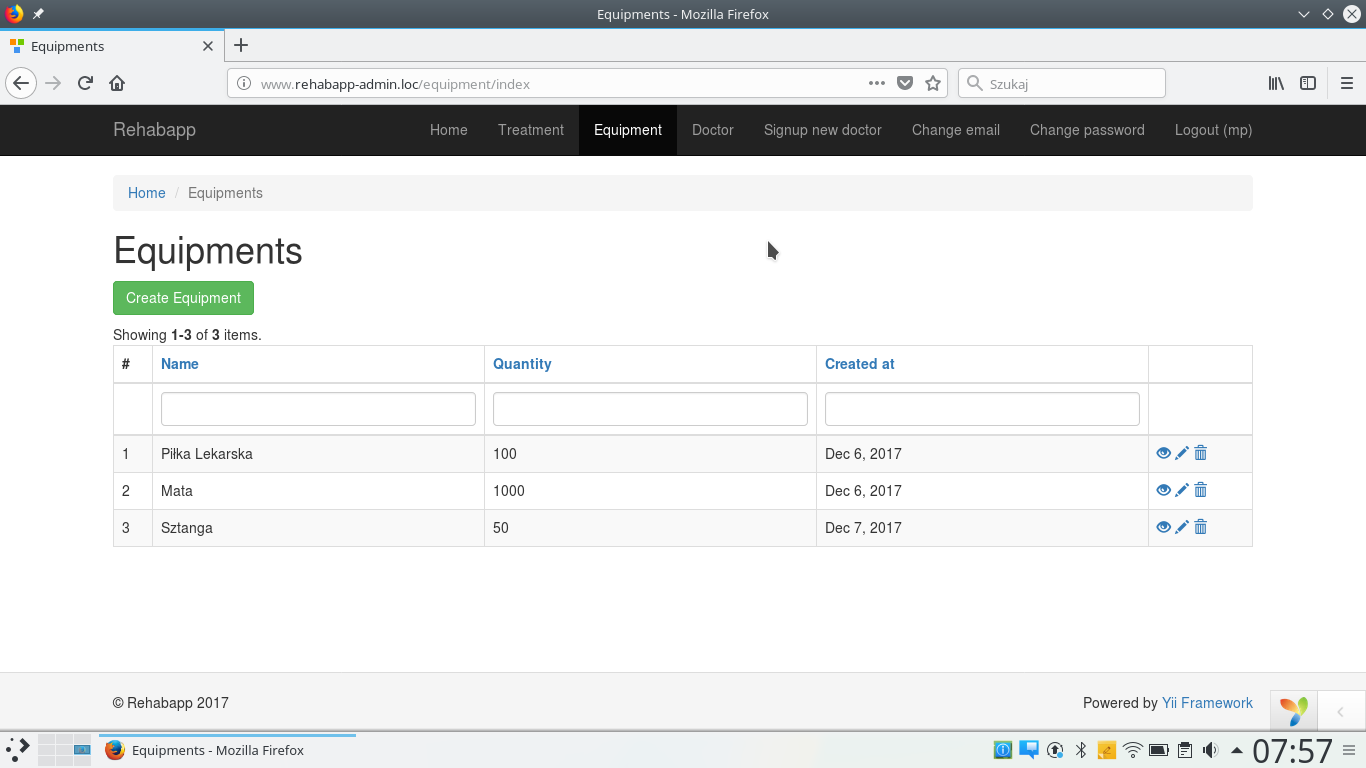
\includegraphics[scale=0.4]{obraz/5.png}
%\begin{center}{\scriptsize Rysunek 1: Diagram przypadków użycia.}\end{center}
\vspace{0,5cm}

\vspace{0,5cm}
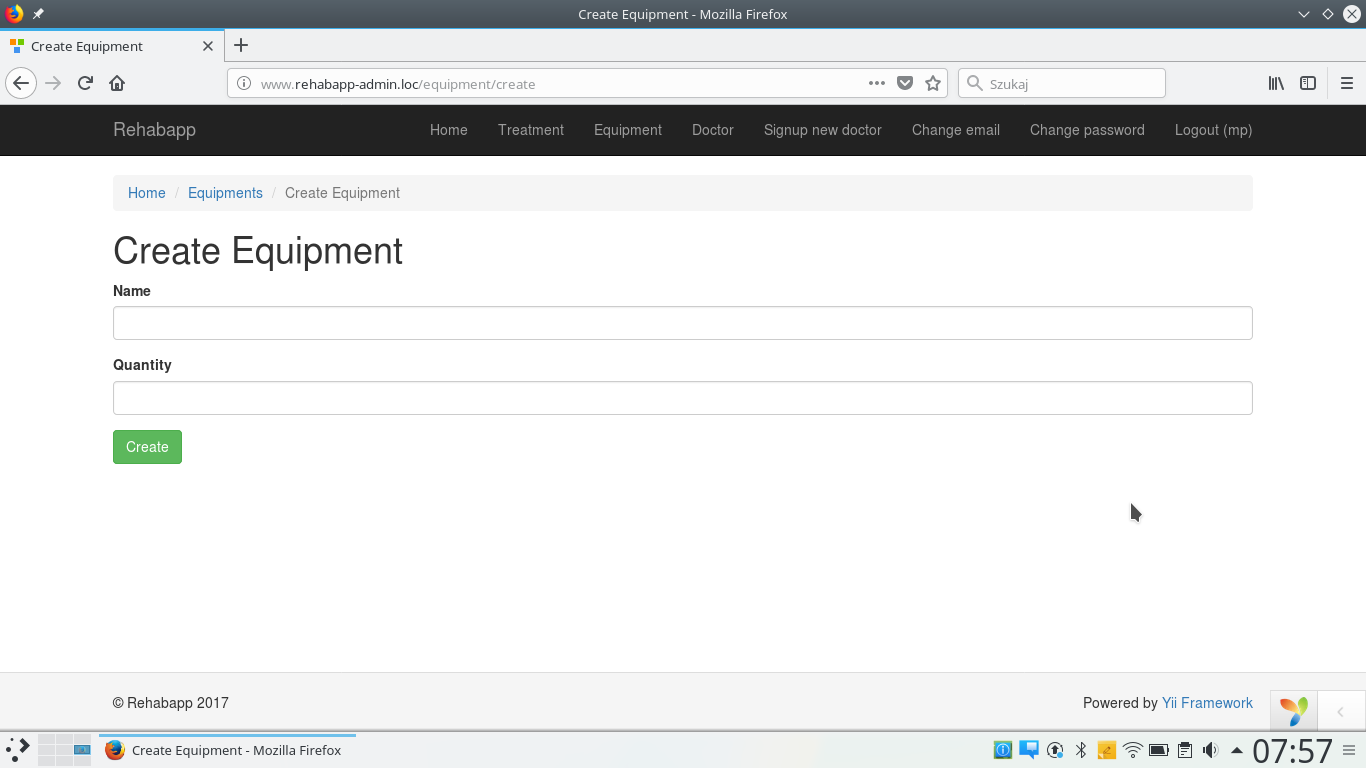
\includegraphics[scale=0.4]{obraz/6.png}
%\begin{center}{\scriptsize Rysunek 1: Diagram przypadków użycia.}\end{center}
\vspace{0,5cm}

\vspace{0,5cm}
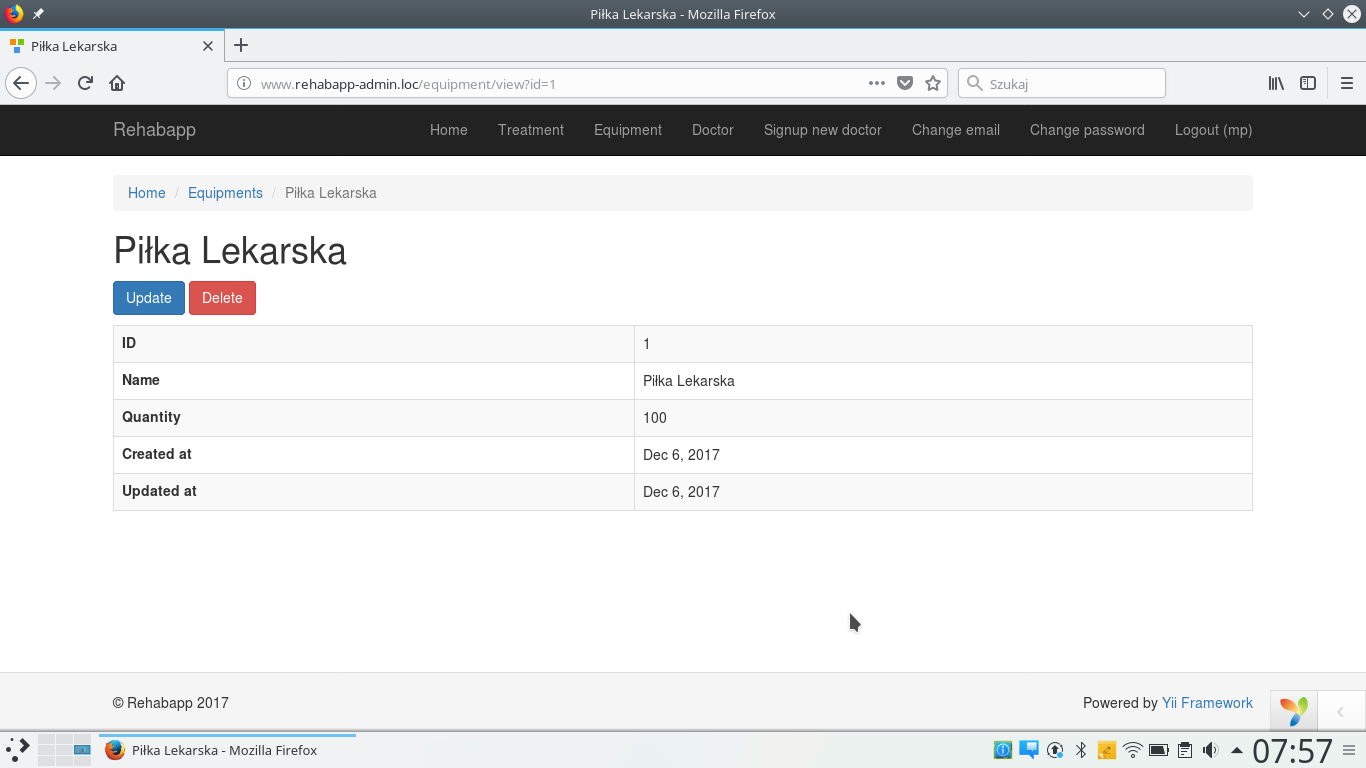
\includegraphics[scale=0.4]{obraz/7.png}
%\begin{center}{\scriptsize Rysunek 1: Diagram przypadków użycia.}\end{center}
\vspace{0,5cm}

\vspace{0,5cm}
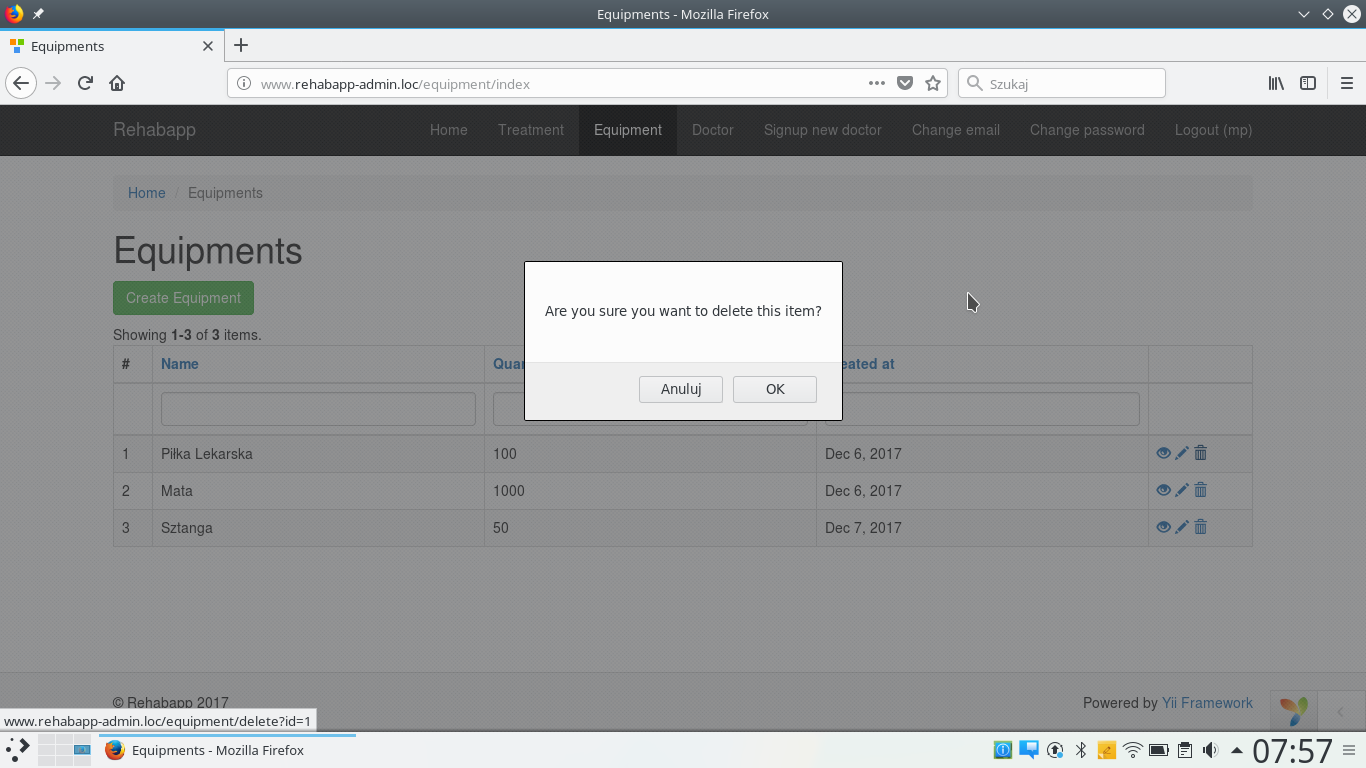
\includegraphics[scale=0.4]{obraz/8.png}
%\begin{center}{\scriptsize Rysunek 1: Diagram przypadków użycia.}\end{center}
\vspace{0,5cm}
\newpage
	\item Uprawnienia administratora umożliwiają również zarządzanie zabiegami. Wszystkie funkcjonalności dotyczące zabiegów w systemie zostały zaimplementowane zgodnie z wymaganiami o numerach od 11 do 15.
	
	
\vspace{0,5cm}
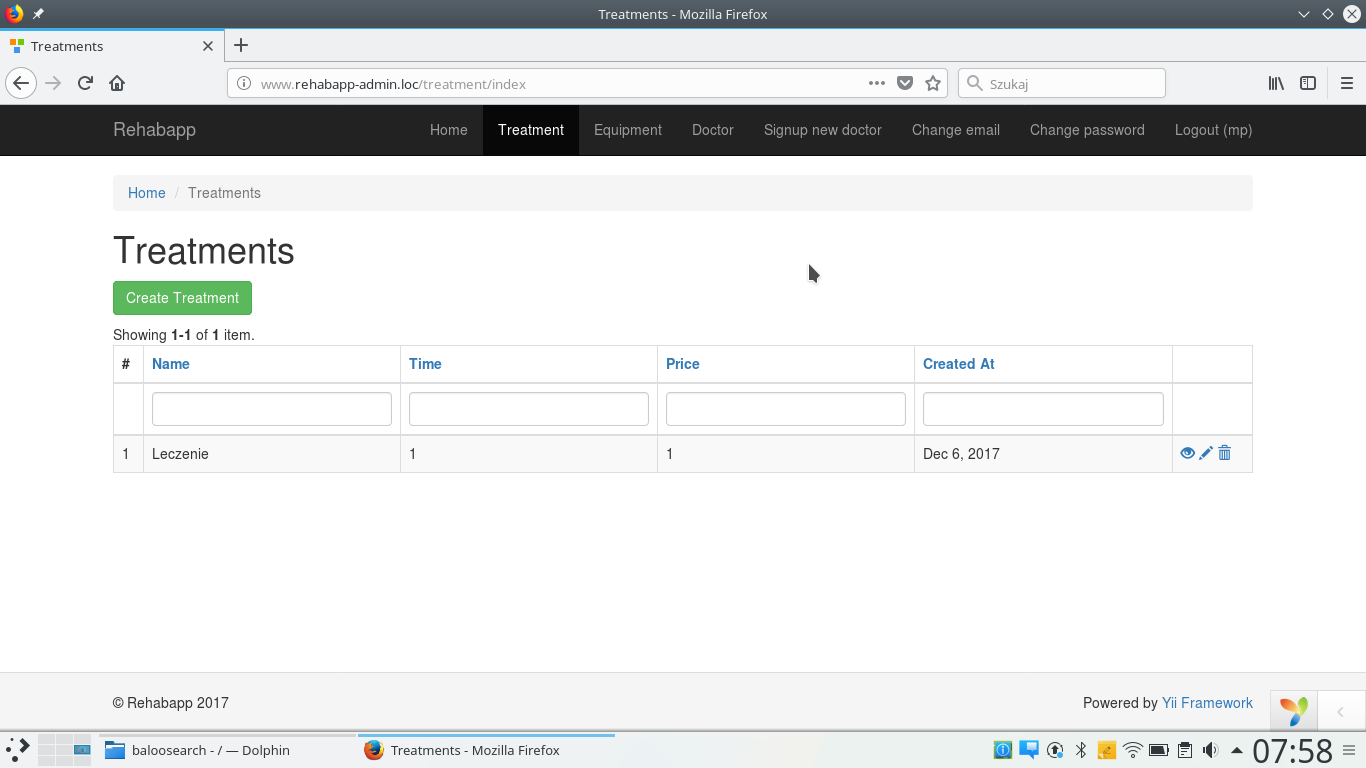
\includegraphics[scale=0.4]{obraz/9.png}
%\begin{center}{\scriptsize Rysunek 1: Diagram przypadków użycia.}\end{center}
\vspace{0,5cm}

\vspace{0,5cm}
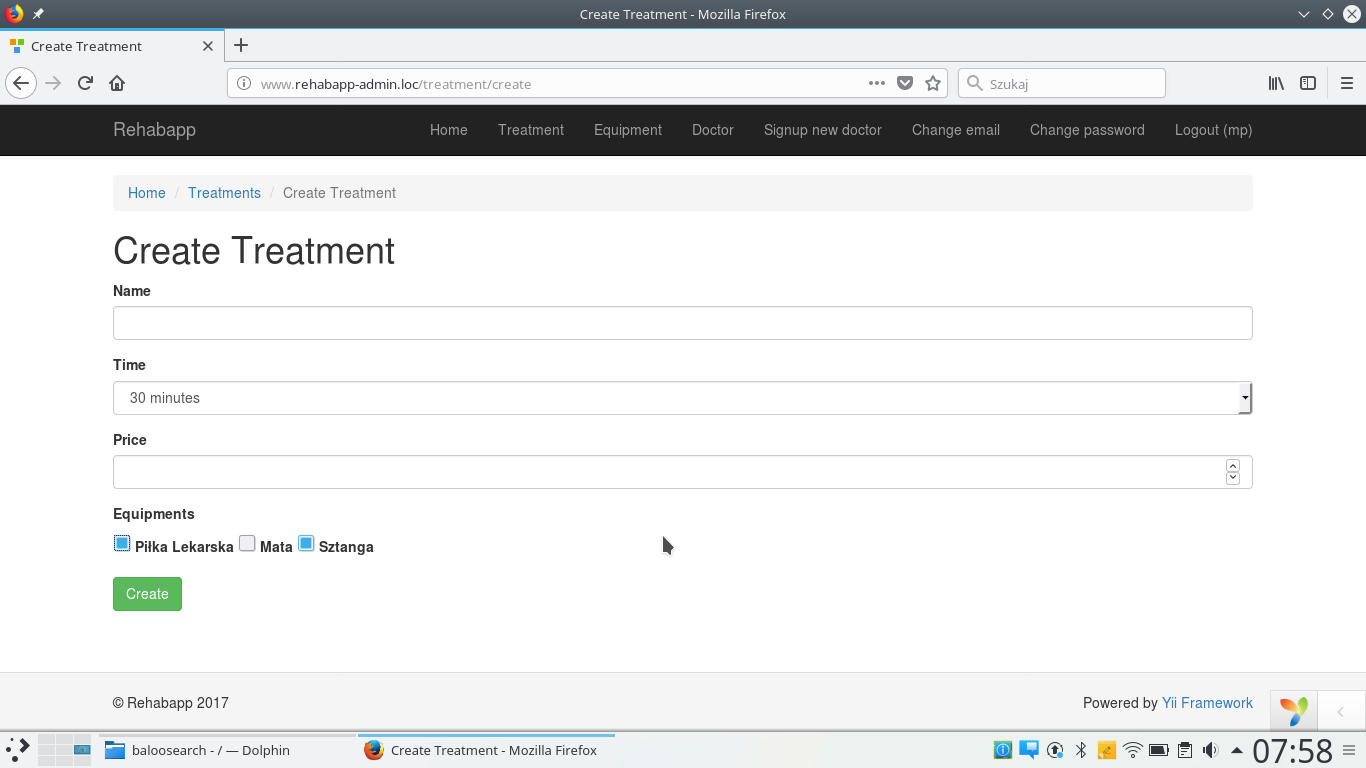
\includegraphics[scale=0.4]{obraz/10.png}
%\begin{center}{\scriptsize Rysunek 1: Diagram przypadków użycia.}\end{center}
\vspace{0,5cm}

\vspace{0,5cm}
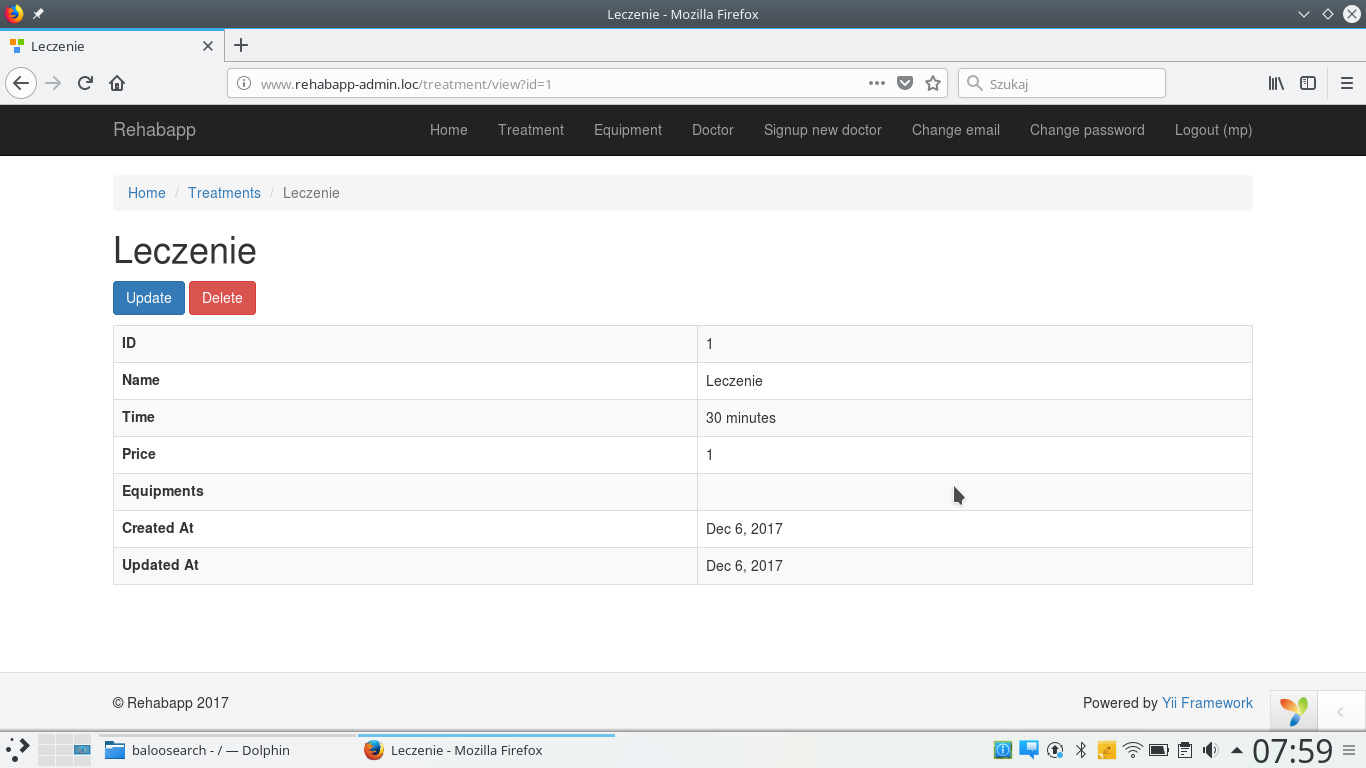
\includegraphics[scale=0.4]{obraz/11.png}
%\begin{center}{\scriptsize Rysunek 1: Diagram przypadków użycia.}\end{center}
\vspace{0,5cm}

\vspace{0,5cm}
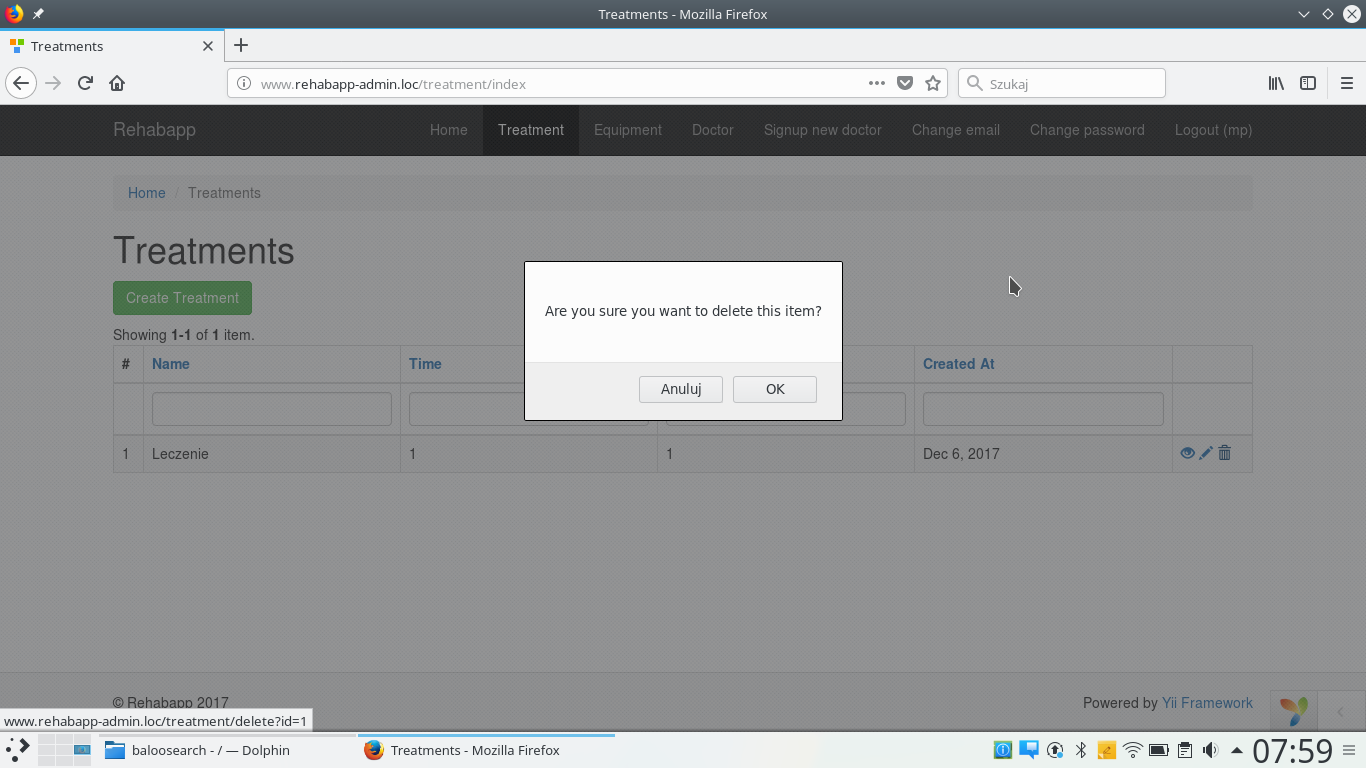
\includegraphics[scale=0.4]{obraz/12.png}
%\begin{center}{\scriptsize Rysunek 1: Diagram przypadków użycia.}\end{center}
\vspace{0,5cm}
\newpage
	\item Administrator ma również możliwość zarządzania (zgodnie z wymaganiami od 16 do 22) inną grupą użytkowników systemów, jaką są lekarze. Czynności tego dotyczące to dodawanie, edycja i usuwanie lekarzy, wyświetlanie listy wszystkich lekarzy pracujących w placówce, wyświetlanie szczegółów dotyczących konkretnego lekarza, a także zmiana hasła i dodawanie terminów wizyt lekarzowi.
	
	
\vspace{0,5cm}
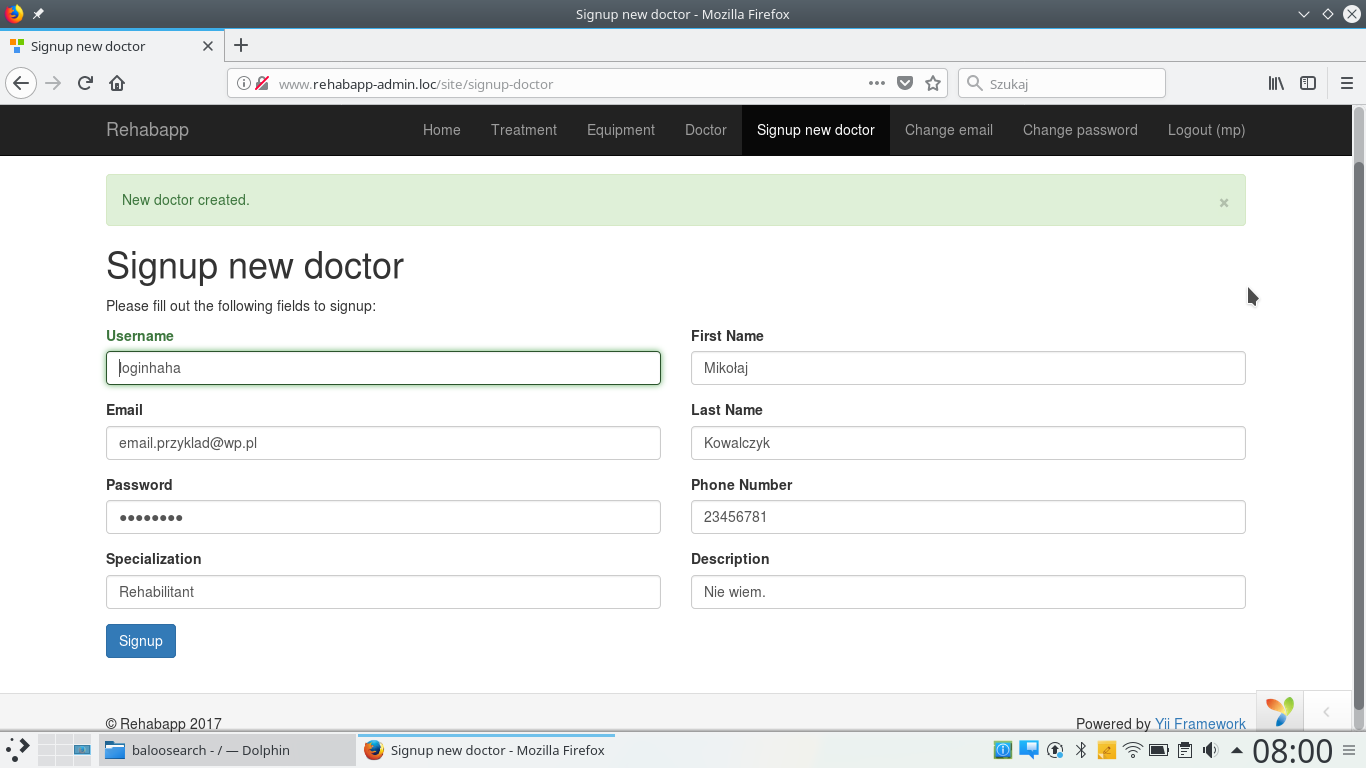
\includegraphics[scale=0.4]{obraz/13.png}
%\begin{center}{\scriptsize Rysunek 1: Diagram przypadków użycia.}\end{center}
\vspace{0,5cm}

\vspace{0,5cm}
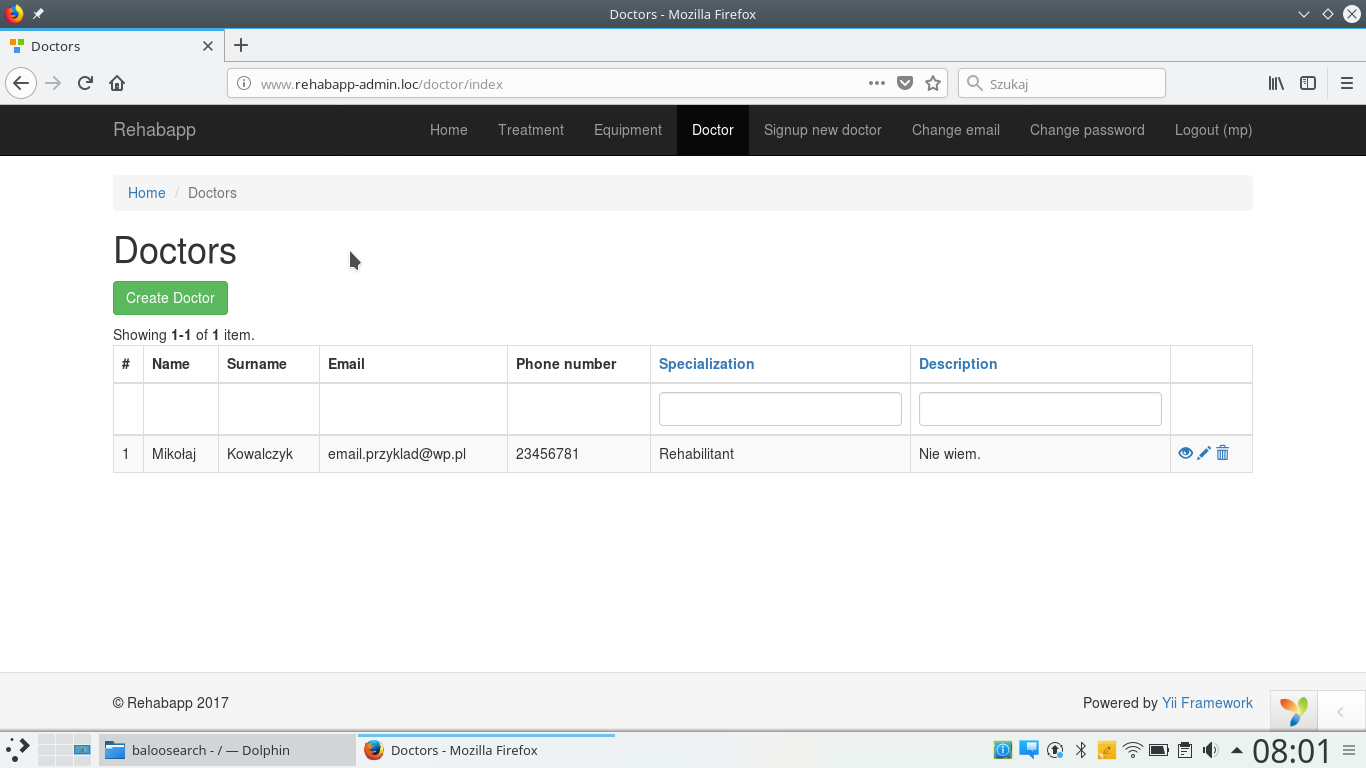
\includegraphics[scale=0.4]{obraz/14.png}
%\begin{center}{\scriptsize Rysunek 1: Diagram przypadków użycia.}\end{center}
\vspace{0,5cm}

\vspace{0,5cm}
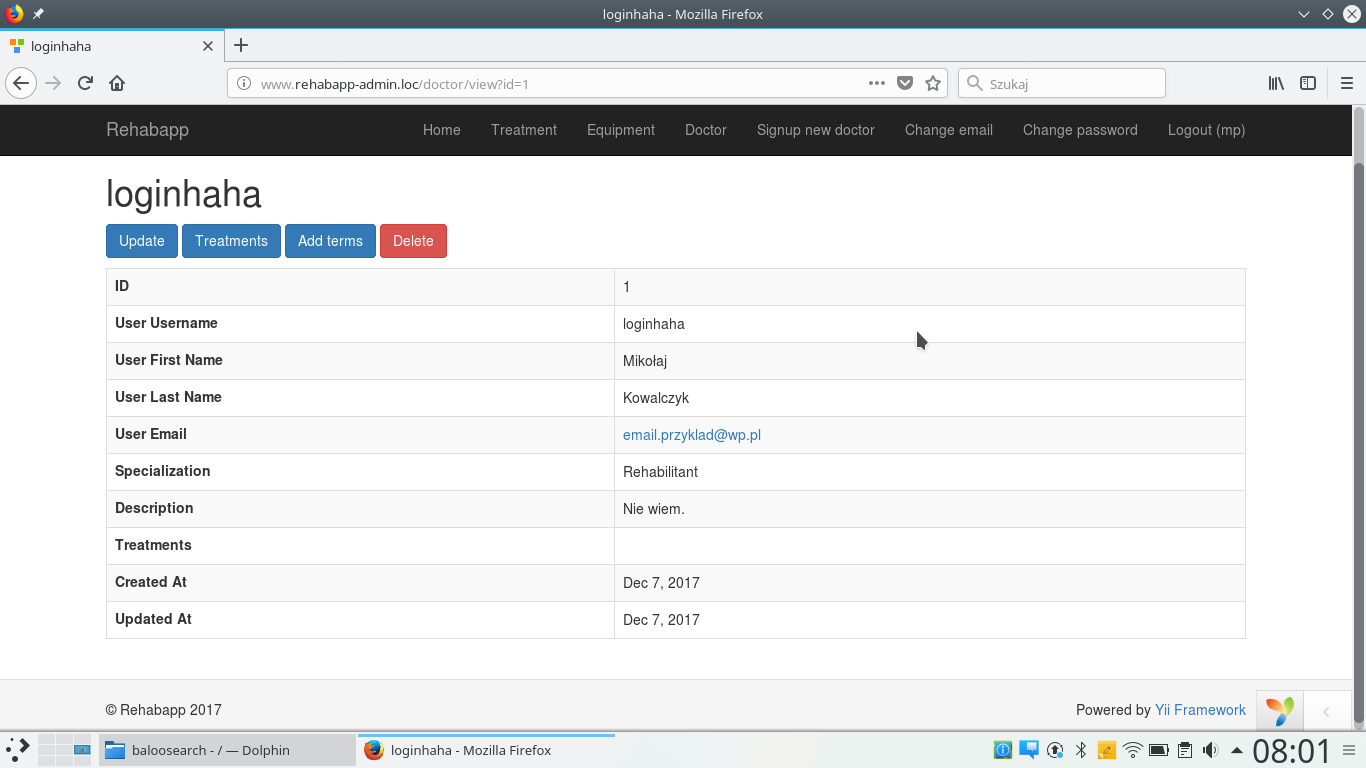
\includegraphics[scale=0.4]{obraz/15.png}
%\begin{center}{\scriptsize Rysunek 1: Diagram przypadków użycia.}\end{center}
\vspace{0,5cm}

\vspace{0,5cm}
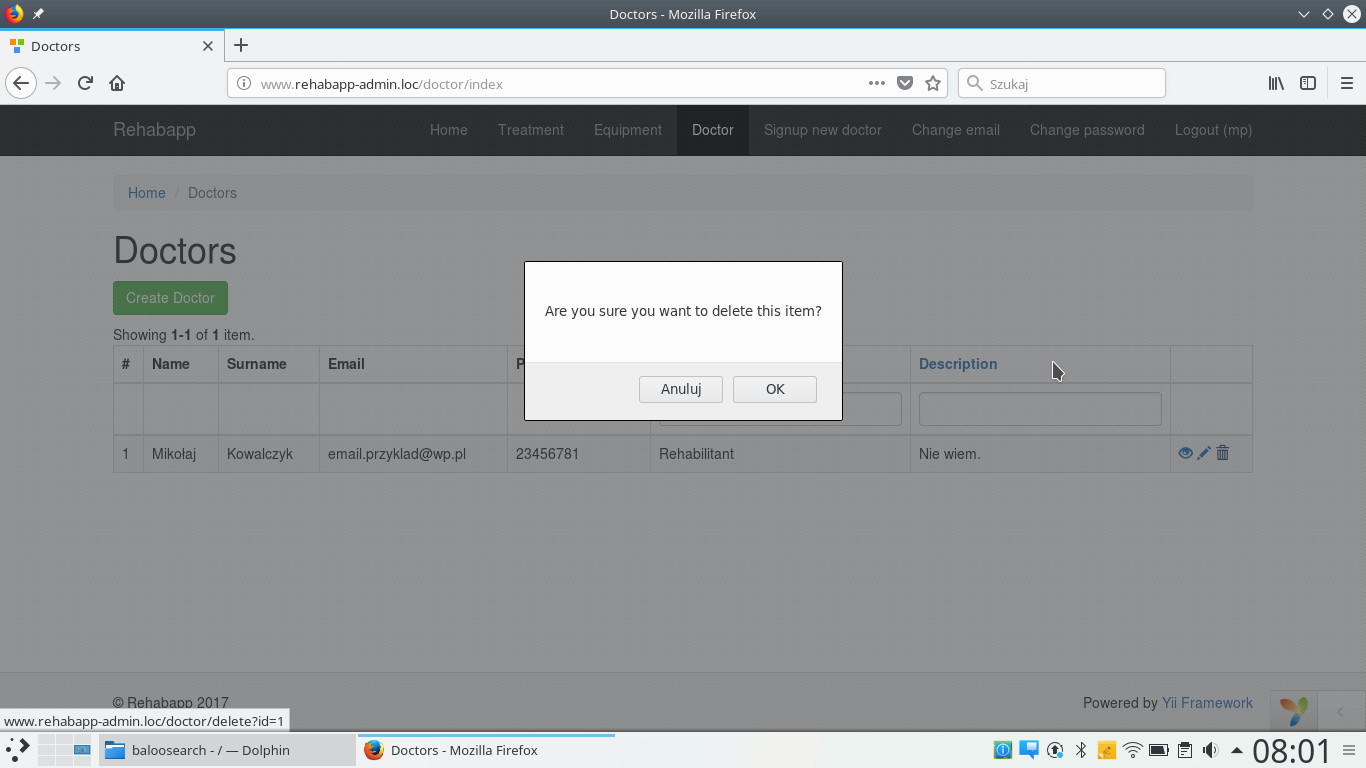
\includegraphics[scale=0.4]{obraz/16.png}
%\begin{center}{\scriptsize Rysunek 1: Diagram przypadków użycia.}\end{center}
\vspace{0,5cm}
	


\end{itemize}
\newpage

\subsection{Moduł pacjenta}



\begin{itemize}
	\item Pacjent w celu korzystania z usług placówki musi posiadać konto w systemie. Zaimplementowane funkcjonalności w oparciu o wymagania od 27 do 32 umożliwiają rejestrację, logowanie, resetowanie i zmianę hasła, zmianę adresu email oraz wylogowanie z systemu.

\vspace{0,5cm}
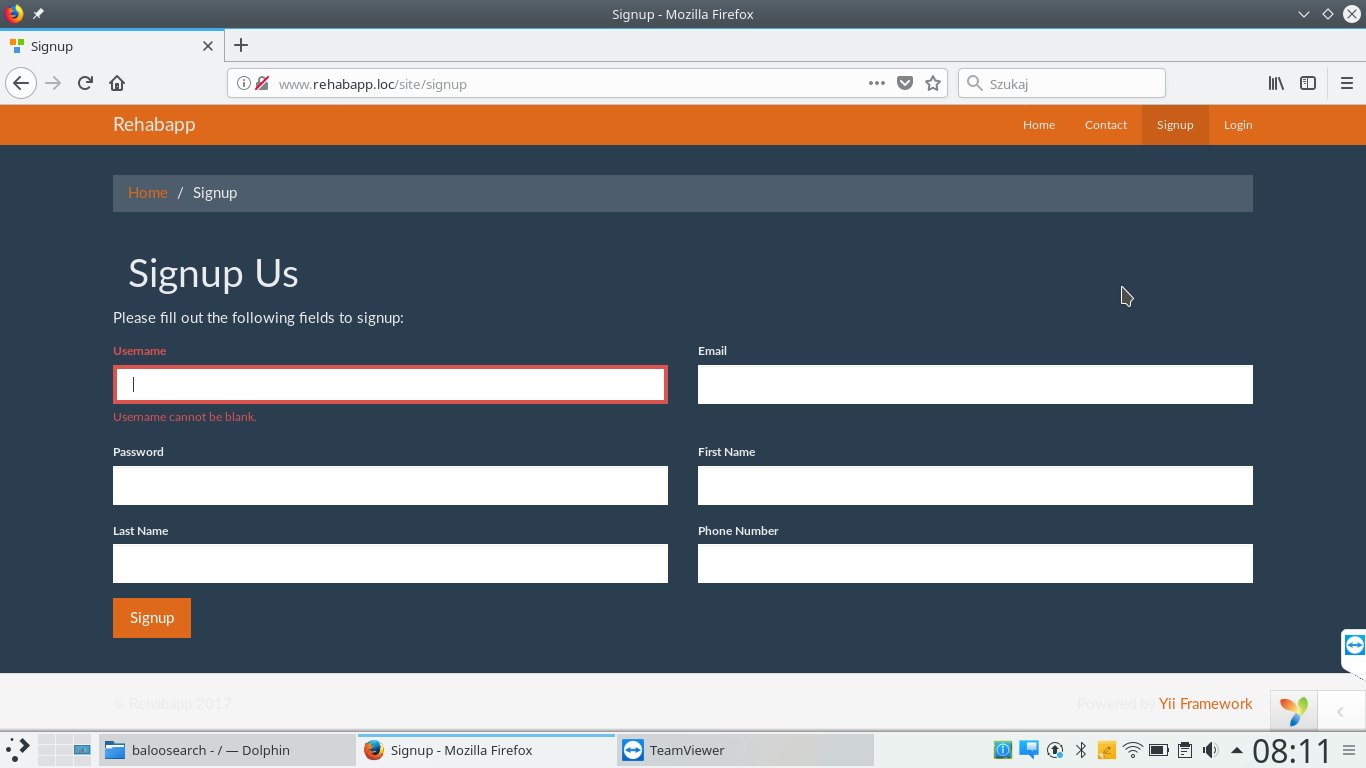
\includegraphics[scale=0.4]{obraz/17.png}
%\begin{center}{\scriptsize Rysunek 1: Diagram przypadków użycia.}\end{center}
\vspace{0,5cm}

\vspace{0,5cm}
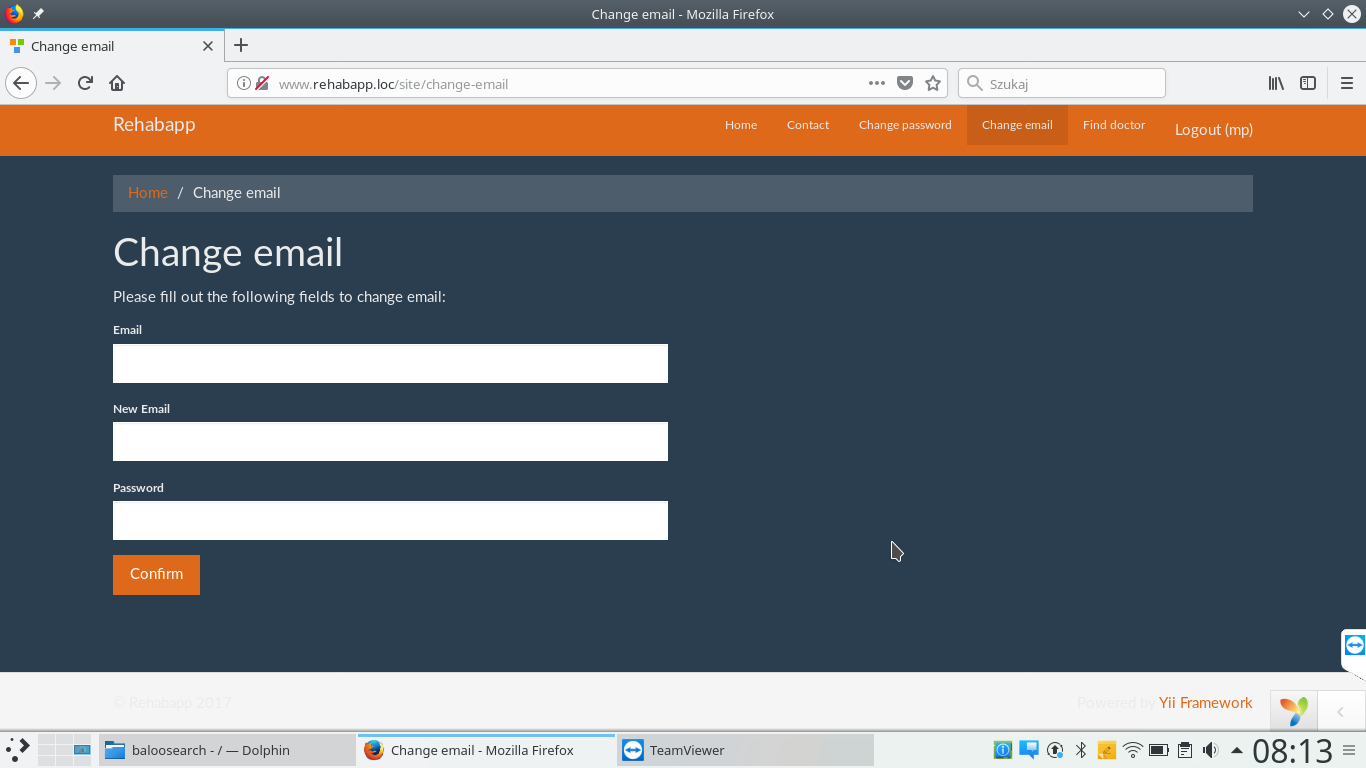
\includegraphics[scale=0.4]{obraz/19.png}
%\begin{center}{\scriptsize Rysunek 1: Diagram przypadków użycia.}\end{center}
\vspace{0,5cm}

\vspace{0,5cm}
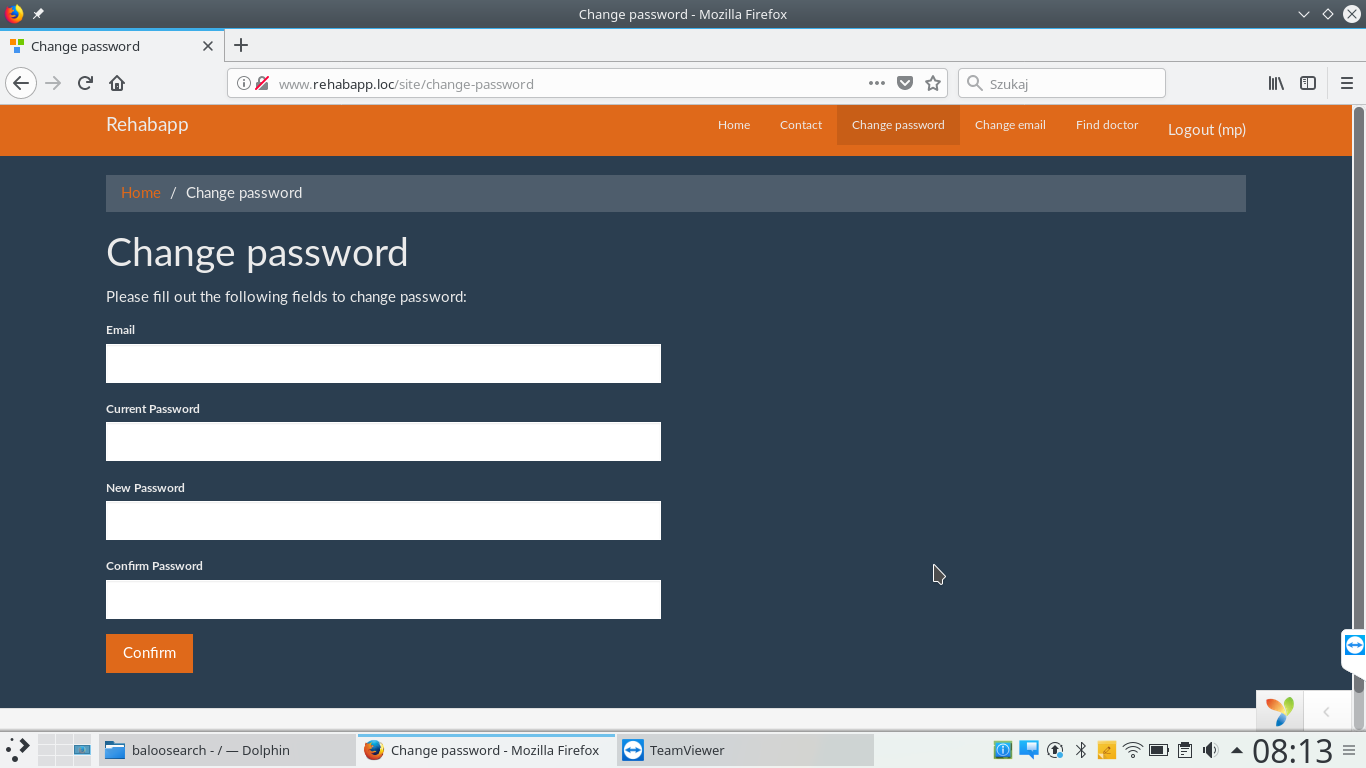
\includegraphics[scale=0.4]{obraz/20.png}
%\begin{center}{\scriptsize Rysunek 1: Diagram przypadków użycia.}\end{center}
\vspace{0,5cm}

	\item Pacjent ma możliwość wyszukiwania lekarzy i wyświetlania ich profili.
	
\vspace{0,5cm}
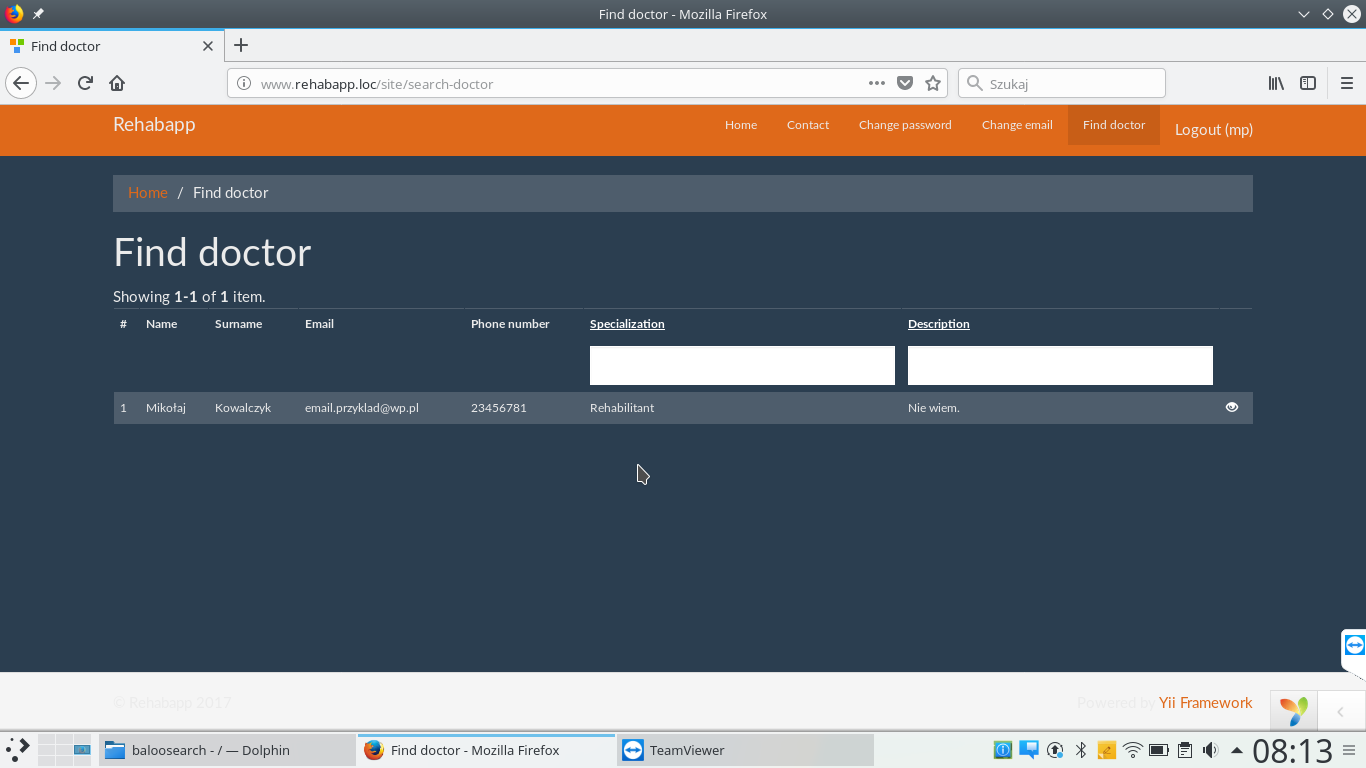
\includegraphics[scale=0.4]{obraz/18.png}
%\begin{center}{\scriptsize Rysunek 1: Diagram przypadków użycia.}\end{center}
\vspace{0,5cm}

\vspace{0,5cm}
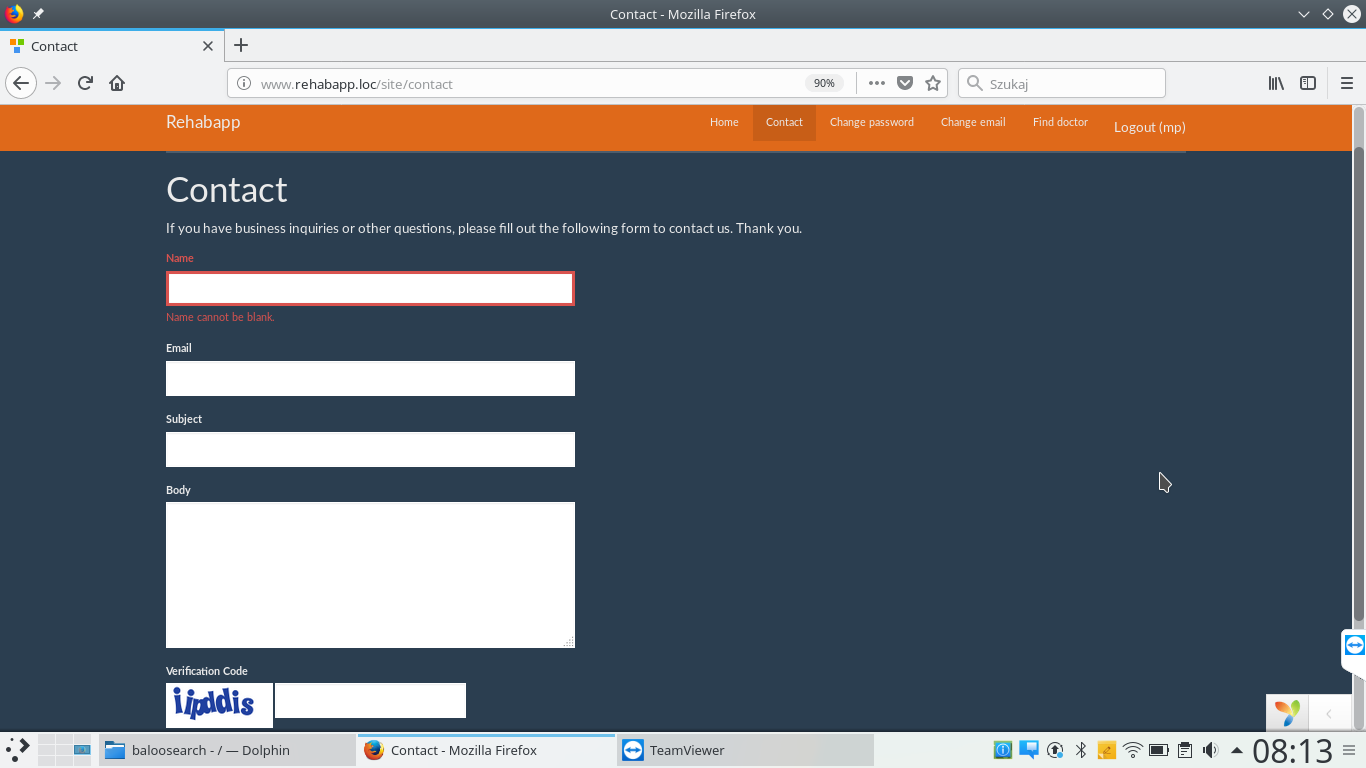
\includegraphics[scale=0.4]{obraz/21.png}
%\begin{center}{\scriptsize Rysunek 1: Diagram przypadków użycia.}\end{center}
\vspace{0,5cm}


\end{itemize}
\newpage
\subsection{Moduł mobilny lekarza}


\begin{itemize}
	\item Do modułu mobilnego, lekarz może zalogować się jedynie po stworzeniu konta w serwisie webowym. 

\vspace{0,5cm}
\begin{center}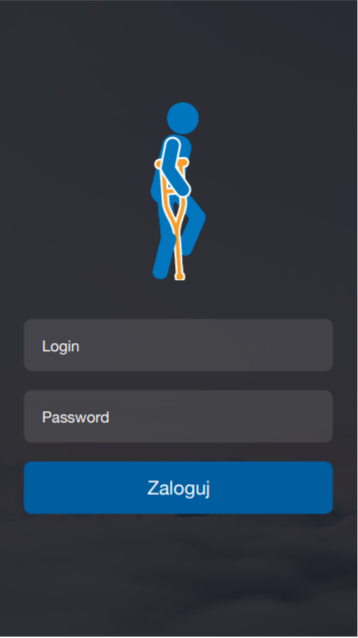
\includegraphics{obraz2/1.png}\end{center}
%\begin{center}{\scriptsize Rysunek 1: Diagram przypadków użycia.}\end{center}
\vspace{0,5cm}

\newpage
	\item Głównym ekranem, jaki widzi lekarz, jest kalendarz, z którego widzi statusy dni pracy (zielony - wszystkie terminy w danym dniu dostępne, żółty - pozostały jeszcze wolne terminy, czerwony - wszystkie terminy w danym dniu zajęte.) 
	
\vspace{0,5cm}
\begin{center}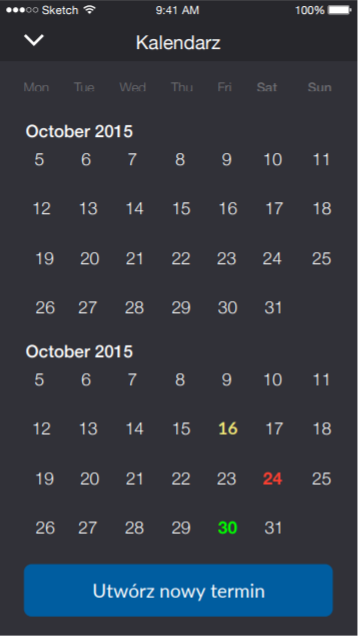
\includegraphics{obraz2/2.png}\end{center}
%\begin{center}{\scriptsize Rysunek 1: Diagram przypadków użycia.}\end{center}
\vspace{0,5cm}
\newpage
	\item Po wciśnięciu przycisku Utwórz nowy termin, otwierany jest panel, z którego można wybrać przedział czasowy trwania zabiegu, jego rodzaj oraz ustalić, czy chcemy, aby zabieg był powtarzany w poszczególnych dniach tygodnia. 
	
\vspace{0,5cm}
\begin{center}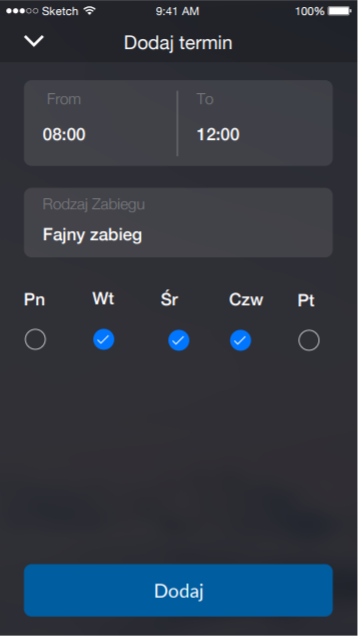
\includegraphics{obraz2/3.png}\end{center}
%\begin{center}{\scriptsize Rysunek 1: Diagram przypadków użycia.}\end{center}
\vspace{0,5cm}
\newpage
	\item Przy wyborze danego dnia z kalendarza, wyświetlany jest spis zabiegów z całego dnia, nazwa, godziny zabiegu oraz status (zajęty, potwierdzony). Z poziomu tego ekranu, możemy przesuwając przycisk z zabiegiem (w lewo - usunąć dany zabieg, w prawo - potwierdzić odbycie się zabiegu). 
	
\vspace{0,5cm}
\begin{center}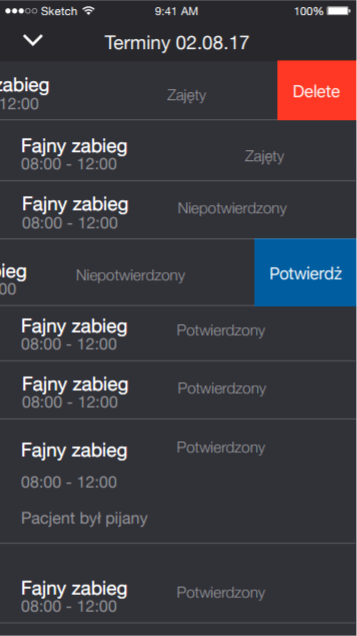
\includegraphics{obraz2/6.png}\end{center}
%\begin{center}{\scriptsize Rysunek 1: Diagram przypadków użycia.}\end{center}
\vspace{0,5cm}
\newpage
	\item Po potwierdzeniu odbycia się zabiegu, wyświetlane jest okienko, w którym możemy wprowadzić krótką notkę dotycząca przebiegu zabiegu.
	
\vspace{0,5cm}
\begin{center}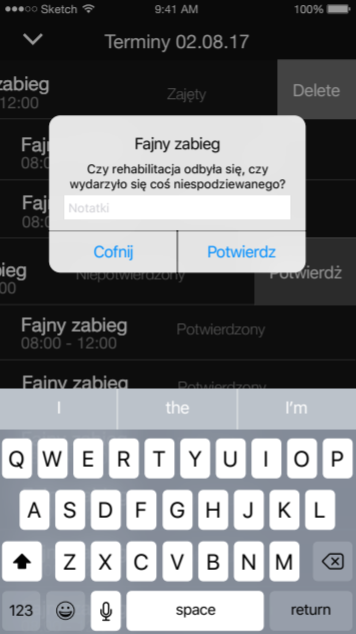
\includegraphics{obraz2/7.png}\end{center}
%\begin{center}{\scriptsize Rysunek 1: Diagram przypadków użycia.}\end{center}
\vspace{0,5cm}
\newpage
	\item Kolejną funkcjonalnością jest lista pacjentów. Z niej lekarz może wyszukać (scrollując lub używając prostego filtra po nazwisku) pacjenta. Z poziomu samej listy widoczne jest imię, nazwisko oraz email pacjenta. 
	
\vspace{0,5cm}
\begin{center}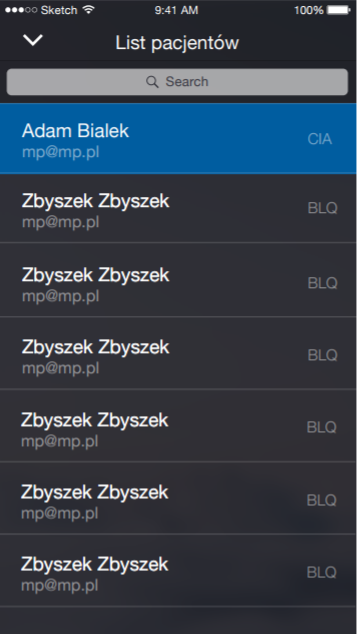
\includegraphics{obraz2/4.png}\end{center}
%\begin{center}{\scriptsize Rysunek 1: Diagram przypadków użycia.}\end{center}
\vspace{0,5cm}
\newpage
	\item Przy wyborze pacjenta z listy, widoczny jest dostęp do historii wizyt. W każdym rekordzie jest nazwa zabiegu, data przeprowadzenia, oraz opcjonalna, krótka notatka. 
	
\vspace{0,5cm}
\begin{center}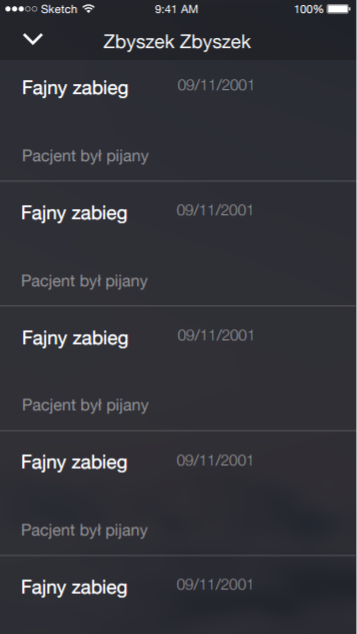
\includegraphics{obraz2/5.png}\end{center}
%\begin{center}{\scriptsize Rysunek 1: Diagram przypadków użycia.}\end{center}
\vspace{0,5cm}






\end{itemize}

\section{Analiza przebiegu projektu}

\subsection{Różnice pomiędzy implementacją a specyfikacją wymagań}


\begin{itemize}
	\item Aplikacja w języku angielskim
	\begin{itemize}
		\item Językiem interfejsu użytkownika jest język angielski. W niesprecyzowanych założeniach początkowych (język aplikacji nie został określony w wymaganiach pozafunkcjonalnych) zakładany był język polski, jednak ze względu na możliwość ewentualnej rozbudowy, przyjęta została nomenklatura angielska.
	\end{itemize}
	\item Moduł kalendarza
	\begin{itemize}
		\item System miał umożliwiać wyświetlanie kalendarza wizyt dla danego lekarza - aby każdy użytkownik systemu mógł przeglądać harmonogram jego pracy. W trakcie prac została przyjęta koncepcja stworzenia listy wraz z dostępnymi terminami wizyt. Zmiana była spowodowana trudnością implementacyjną pierwotnego założenia.
	\end{itemize}
	
		\item Rejestracja pacjentów i historia pacjenta
	\begin{itemize}
		\item System miał umożliwiać rejestrację pacjenta na wizyty - z powodów terminowych funkcjonalność nie została ukończona i udostępniona. Co za tym idzie - użytkownik nie ma możliwości wglądu do swojej historii.
	\end{itemize}
	


\end{itemize}


\subsection{Odchylenia w realizacji planowanych zadań}

\begin{itemize}

	\item Spotkania grupy projektowej
	\begin{itemize}
		\item Z założenia, grupa projektowa miała się spotykać cyklicznie i razem opracowywać powierzone zadania. Z powodu rozbieżności w planach zajęć, trudno było wyznaczyć termin, który pasowałby każdemu członkowi zespołu.
	\end{itemize}
	\item Plan komunikacji
		\begin{itemize}
		\item Początkowy plan komunikacji zakładał największy przepływ informacji przez portale społecznościowe, rozmowy telefoniczne. Z biegiem czasu, okazało się, że najefektywniejszą formą przekazywania założeń oraz analizy zadań, są spotkania grupowe.
	\end{itemize}
	
		\item Podział modułowy
		\begin{itemize}
		\item W zespole funkcjonowały podgrupy - każda z nich miała określone zadania do wykonania, opisane w dokumentacji. Z powodu braku wystarczającej znajomości niektórych technologii przez niektórych członków grupy, część zadań była realizowana “płynnie” między zespołami.
	\end{itemize}
	
		\item Realizacja funkcjonalności
		\begin{itemize}
		\item Z racji tego, iż niektóre rozwiązania funkcjonalne były bliźniaczo podobne (na przykład w module pacjenta jak i administratora), część z nich, po modyfikacjach, była wykorzystywana w innych modułach.
	\end{itemize}
	
\end{itemize}


\newpage
\subsection{Przewidziane oraz nieprzewidziane problemy}

\subsubsection{Przewidziane problemy}

\begin{itemize}
	\item Brak znajomości wykorzystywanego środowiska oraz języków programowania
	\begin{itemize}
		\item Ze względu na to, iż projekt tworzony był w grupie 6-osobowej, należało dojść do kompromisu w sprawie wykorzystywanych technologii - nie każdy członek grupy specjalizuje się w tym samym języku programowania/dziedzinie. Z tego powodu, pojawiały się różne problemy - począwszy od konfuguracji środowiska, po brak zrozumienia niektórych mechanizmów składniowych języka/języków.
	\end{itemize}
	\item Brak wystarczającej ilości czasu
	\begin{itemize}
		\item Projekt realizowany był na 7 semestrze studiów inżynierskich - co za tym idzie, każdy członek grupy, równolegle, zobowiązany był do pisania własnej pracy dyplomowej oraz innych projektów w ramach semestru.
	\end{itemize}
	\item Złożoność projektu
	\begin{itemize}
		\item Zadanie zaprojektowania oraz wykonania aplikacji do zarządzania dniem pracy specjalistów nie należało do najłatwiejszych. Decydując się na taki projekt, grupa musiała zdawać sobie sprawę z jego rozpiętości i złożoności.
	\end{itemize}
\end{itemize}

\subsubsection{Nieprzewidziane problemy}

\begin{itemize}
	\item Problemy sprzętowe
	\begin{itemize}
		\item W fazie projektowania systemu, u dwóch członków zespołu, pojawiły się poważne problemy związane z niezbędnymi narzędziami pracy. Przez to grupa projektowa była mniej wydajna, a praca została na pewien czas wstrzymana. 
	\end{itemize}
	\item Problemy zdrowotne
	\begin{itemize}
		\item W okresie jesiennym odporność organizmu człowieka wyraźnie spada, narażając na przeziębienie i grypę. Stanom tym towarzyszą często inne jesienne objawy – bóle głowy, ból gardła czy ogólne osłabienie, które negatywnie wpływają na efektywność pracy.
	\end{itemize}
	\item Nieprzewidziana złożoność przewidzianych problemów
	\begin{itemize}
		\item Niektóre przewidziane utrudnienia w tworzeniu projektu okazały się zdecydowanie poważniejsze, niż zakładano. W szczególności krótki czas realizacji przy tak złożonym projekcie.
	\end{itemize}
\end{itemize}

\section{Możliwości dalszego rozwoju projektu}



\begin{itemize}
	\item Dokończenie wszystkich funkcjonalności.
	\begin{itemize}
		\item Z racji niewystarczającej ilości czasu, nie wszystkie funkcjonalności zostały wykonane bądź dopracowane. 
	\end{itemize}
	
	\item Estetyka aplikacji.
	\begin{itemize}
		\item Nadrzędnym celem było stworzenie wszystkich modułów oraz dopracowanie komunikacji między nimi. Interfejs serwisu jest przyjazny dla użytkownika oraz intuicyjny - jednak na jego stworzenie nie została poświęcona odpowiednia ilość czasu, a co za tym idzie - pojawiają się niedociągnięcia, które należałoby poprawić.
	\end{itemize}
	
		\item Moduł mobilny dla pacjenta.
	\begin{itemize}
		\item W ramach projektu został stworzony jeden moduł mobilny dla jednego aktora - lekarza. Kolejną możliwością rozbudowy aplikacji jest dostarczenie drugiego, przeznaczonego dla pacjenta.
	\end{itemize}

\end{itemize}

\end{document}
